

\begin{enumerate}[label=\thesubsection.\arabic*, ref=\thesubsection.\theenumi]

\item Let $A$ be a scalar matrix of order $3$ such that the sum
of all its elements is $9$. Find the product of all the
elements of $A$.

\begin{enumerate}
\begin{multicols}{4}
    \item $9$
    \item $27$
    \item $3$
    \item $0$
\end{multicols}
\end{enumerate}
\solution
Since $A$ is a scalar matrix of order $3$, it can be
written as
\begin{align}
A =
\myvec{
a & 0 & 0 \\
0 & a & 0 \\
0 & 0 & a
}
\end{align}

Given that the sum of all the elements is $9$,
\begin{align}
a+a+a=9\\
3a=9\\
a=3
\end{align}

Therefore, the matrix is
\begin{align}
A =
\myvec{
3 & 0 & 0 \\
0 & 3 & 0 \\
0 & 0 & 3
}
\end{align}

The product of all the elements is
\begin{align}
3 \times 0 \times 0 \times
0 \times 3 \times 0 \times
0 \times 0 \times 3=0
\end{align}
Hence, the correct answer is
\begin{align}
\text{Option \brak{D}: }0
\end{align}


\item 
Let $f:[0,\infty)\rightarrow[-5,\infty)$ be defined by
\begin{align}
f\brak{x}=9x^2+6x-5.
\end{align}

Then $f$ is

\begin{enumerate}
    \item one-one but not onto
    \item onto but not one-one
    \item both one-one and onto
    \item neither one-one nor onto

\end{enumerate}

\solution
Given,
\begin{align}
f\brak{x}=9x^2+6x-5,\qquad x=0.
\end{align}


{Step 1: Check whether the function is one-one.}

Differentiating with respect to $x$,
\begin{align}
f'\brak{x}=18x+6.
\end{align}


Since $x=0$,
\begin{align}
18x+6>0.
\end{align}

Therefore, $f\brak{x}$ is strictly increasing on
$[0,\infty)$.
\\Hence, $f$ is a one-one function.
\\{Step 2: Check whether the function is onto.}
\\At $x=0$,
\begin{align}
f\brak{0}=9\brak{0}^2+6\brak{0}-5=-5.
\end{align}
Also,
\begin{align}
\lim_{x\to\infty}f\brak{x}=\infty.
\end{align}
Since $f$ is continuous and strictly increasing on
$[0,\infty)$, its range is
\begin{align}
\operatorname{Range}\brak{f}=[-5,\infty).
\end{align}
The range of $f$ is equal to its codomain. Therefore,
$f$ is onto.

{Conclusion:}
\\The function is both one-one and onto.
\\Hence, the correct answer is
\begin{align}
\text{Option \brak{C}: Both one-one and onto}
\end{align}


\item
If
\begin{align}
\mydet{
-a & a & a\\
b & -b & b\\
c & c & -c
}
= kabc,
\end{align}
then the value of $k$ is
\begin{enumerate}
\begin{multicols}{4}
    \item $0$
    \item $1$
    \item $2$
    \item $4$
\end{multicols}
\end{enumerate}

\solution
Given,
\begin{align}
\mydet{
-a & a & a\\
b & -b & b\\
c & c & -c
}
= kabc,
\end{align}
Taking $a$, $b$, and $c$ common from the first,
second, and third rows respectively, we get

\begin{align}
=abc
\mydet{
-1 & 1 & 1\\
1 & -1 & 1\\
1 & 1 & -1
}
\end{align}
using the \eqref{eq:EE26BTECH11211-Prob_1} expanding the determinant.
\begin{align}
=abc\left[
\brak{-1}\brak{1-1}
-\brak{ -1-1}
+\brak{1+1}
\right].
&=abc[0+2+2]
&=4abc.
\end{align}
Comparing this result with $kabc$, we obtain
\begin{align}
kabc=4abc.
\end{align}

Therefore,

\begin{align}
k=4
\end{align}
Hence, the correct answer is

\item
The number of points at which the function
\[
f\brak{x}=
\begin{cases}
|x|+3, & x\leq -3,\\
-2x, & -3<x<3,\\
6x+2, & x= 3
\end{cases}
\]
is discontinuous is

\begin{enumerate}
\begin{multicols}{4}
    \item $0$
    \item $1$
    \item $2$
    \item $3$
    \end{multicols}
\end{enumerate}
\solution
\\The function is defined by three different expressions.
We check continuity at the points where the definition changes:
$x=-3$ and $x=3$.
\\{Step 1: Check continuity at $x=-3$.}
\\The left-hand limit is
\begin{align}
\lim_{x\to-3^-}f\brak{x}
=|-3|+3=6.
\end{align}
The right-hand limit is
\begin{align}
\lim_{x\to-3^+}f\brak{x}
=-2\brak{-3}=6.
\end{align}
The function value is
\begin{align}
f\brak{-3}=|-3|+3=6.
\end{align}
Therefore,
\begin{align}
\lim_{x\to-3^-}f\brak{x}
=\lim_{x\to-3^+}f\brak{x}=f\brak{-3}.
\end{align}
Hence, $f$ is continuous at $x=-3$.
\\{Step 2: Check continuity at $x=3$.}
\\The left-hand limit is
\begin{align}
\lim_{x\to3^-}f\brak{x}=-2\brak{3}=-6.
\end{align}
The right-hand limit is
\begin{align}
\lim_{x\to3^+}f\brak{x}=6\brak{3}+2=20.
\end{align}
The function value is
\begin{align}
f\brak{3}=6\brak{3}+2=20.
\end{align}
Since
\begin{align}
\lim_{x\to3^-}f\brak{x}
\neq
\lim_{x\to3^+}f\brak{x},
\end{align}
the function is discontinuous at $x=3$.
\\{Conclusion:}
\\The function has exactly one point of discontinuity.
\\The following code generates the figure
\begin{lstlisting}[frame=single, basicstyle=\rmfamily, escapeinside={(*@}{@*)}]
(*@\makebox[\dimexpr\linewidth-2\fboxsep-2\fboxrule\relax][c]{codes/s124.py}@*)
\end{lstlisting}
\begin{figure}[ht]
    \centering

    \begin{tikzpicture}
        \node[inner sep=0pt] at (0,0)
        {
            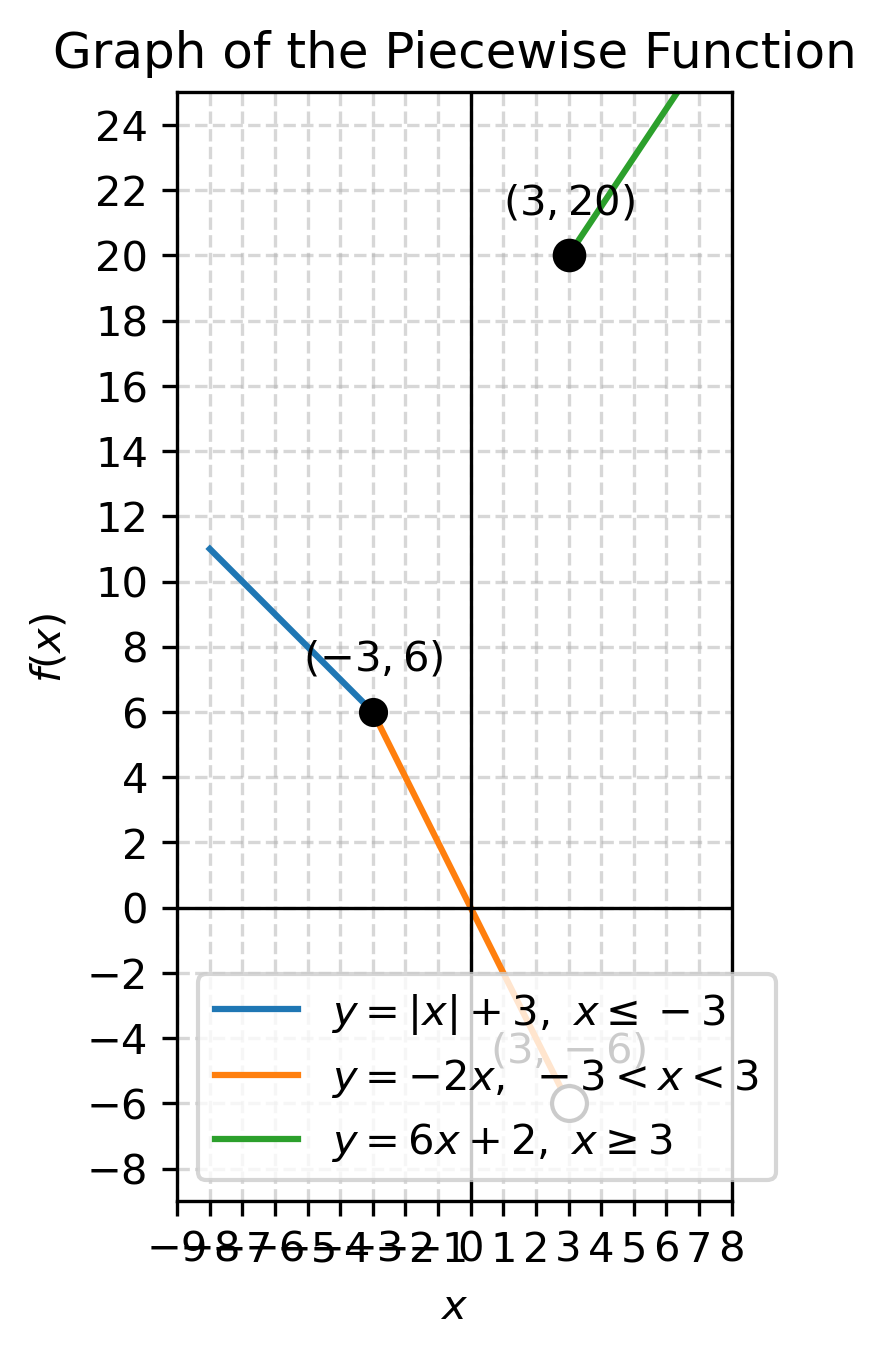
\includegraphics[
                width=0.5\textwidth,
                keepaspectratio
            ]{figs/s124.png}
        };
    \end{tikzpicture}

\end{figure}
\newpage
\item
The function
\begin{align}
f\brak{x}=x^3-3x^2+12x-18
\end{align}
is

\begin{enumerate}
    \item strictly decreasing on $\mathbb{R}$
    \item strictly increasing on $\mathbb{R}$
    \item neither increasing nor decreasing on $\mathbb{R}$
    \item a constant function on $\mathbb{R}$
\end{enumerate}

\solution
Given,
\begin{align}
f\brak{x}=x^3-3x^2+12x-18.
\end{align}

Differentiating with respect to $x$, we obtain
\begin{align}
f'\brak{x}=3x^2-6x+12.
\end{align}

Taking $3$ common,
\begin{align}
f'\brak{x}=3\brak{x^2-2x+4}.
\end{align}

Completing the square,
\begin{align}
f'\brak{x}=3\left[\brak{x-1}^2+3\right].
\end{align}
Since
\begin{align}
\brak{x-1}^2=0,
\end{align}
we have
\begin{align}
\brak{x-1}^2+3>0.
\end{align}

Therefore,
\begin{align}
f'\brak{x}>0
\qquad \text{for all }x\in\mathbb{R}.
\end{align}
Since the derivative is positive throughout $\mathbb{R}$,
the function is strictly increasing on $\mathbb{R}$.

\item
Evaluate
\begin{align}
I=\int_0^{\pi/2}
\frac{\sin x-\cos x}{1+\sin x\cos x}\,dx.
\end{align}

\begin{enumerate}
\begin{multicols}{4}
    \item[\brak{A}] $1$
    \item[\brak{B}] $0$
    \item[\brak{C}] $-1$
    \item[\brak{D}] $\dfrac{\pi}{2}$
\end{multicols}
\end{enumerate}

\solution
Given,
\begin{align}
I=\int_0^{\pi/2}
\frac{\sin x-\cos x}{1+\sin x\cos x}\,dx.
\end{align}
Using the substitution
\begin{align}
x=\frac{\pi}{2}-t,
\end{align}
we have
\begin{align}
dx=-dt.
\end{align}

When $x=0$, $t=\dfrac{\pi}{2}$.

When $x=\dfrac{\pi}{2}$, $t=0$.

Also,
\begin{align}
\sin x=\cos t,\qquad
\cos x=\sin t.
\end{align}

Therefore,
\begin{align}
I=\int_0^{\pi/2}
\frac{\cos t-\sin t}{1+\sin t\cos t}\,dt.
\end{align}

Rewriting the variable $t$ as $x$,
\begin{align}
I=\int_0^{\pi/2}
\frac{\cos x-\sin x}{1+\sin x\cos x}\,dx.
\end{align}
Comparing this with the original integral,
\begin{align}
I=-I.
\end{align}
Hence,
\begin{align}
2I=0
\end{align}
Therefore,
\begin{align}
I=0.
\end{align}

\item
Which of the following differential equations is a
homogeneous differential equation?

\begin{enumerate}
    \item $\displaystyle \frac{dy}{dx}=\cos x-\sin\brak{\frac{x}{y}}$
    \item $\displaystyle \frac{dy}{dx}=\frac{x+y}{x-y}$
    \item $\displaystyle \frac{dy}{dx}=x+y$
    \item $\displaystyle \frac{dy}{dx}=x^2+y^2$
\end{enumerate}

\solution
A first-order differential equation of the form
\begin{align}
\frac{dy}{dx}=F\brak{x,y}
\end{align}
is homogeneous if $F\brak{x,y}$ can be expressed as a
function of $\dfrac{y}{x}$ alone.
For option \brak{B},
\begin{align}
\frac{dy}{dx}=\frac{x+y}{x-y}.
\end{align}

Dividing the numerator and denominator by $x$, we get
\begin{align}
\frac{dy}{dx}
=\frac{1+\dfrac{y}{x}}{1-\dfrac{y}{x}}.
\end{align}
The right-hand side is a function of $\dfrac{y}{x}$
alone.
\\Therefore, the differential equation in option \brak{B}
is homogeneous.

\item
For any two vectors $\vec{a}$ and $\vec{b}$, which of
the following statements is always true?

\begin{enumerate}
    \item $\vec{a}\cdot\vec{b}
    =|\vec{a}|+|\vec{b}|$
    \item $\vec{a}\cdot\vec{b}
    = |\vec{a}|\,|\vec{b}|$   
    \item $\vec{a}\cdot\vec{b}
    \leq |\vec{a}|\,|\vec{b}|$    
    \item $\vec{a}\times\vec{b}
    =|\vec{a}|\,|\vec{b}|$
\end{enumerate}

\solution
The dot product of two vectors is given by\eqref{eq:EE26BTECH11211-Prob_7.1}
\begin{align}
\vec{a}\cdot\vec{b}
=|\vec{a}|\,|\vec{b}|\cos\theta,
\end{align}
where $\theta$ is the angle between the vectors.
Since
\begin{align}
-1\leq\cos\theta\leq1,
\end{align}
we obtain
\begin{align}
-|\vec{a}|\,|\vec{b}|
\leq\vec{a}\cdot\vec{b}
\leq|\vec{a}|\,|\vec{b}|.
\end{align}
Therefore,
\begin{align}
\vec{a}\cdot\vec{b}
\leq|\vec{a}|\,|\vec{b}|.
\end{align}

\item
The foot of the perpendicular drawn from the point
$P\brak{0,1,2}$ to the $x$-axis is

\begin{enumerate}
\begin{multicols}{4}
    \item $\brak{0,1,0}$
    \item $\brak{0,0,2}$
    \item $\brak{1,0,0}$
    \item $\brak{0,0,0}$
\end{multicols}
\end{enumerate}

\solution
Let the given point be
\begin{align}
P=\brak{0,1,2}.
\end{align}

Any point on the $x$-axis has coordinates
\begin{align}
Q=\brak{x,0,0}.
\end{align}
The direction vector of the $x$-axis is
\begin{align}
\vec{d}=\brak{1,0,0}.
\end{align}
Since $PQ$ is perpendicular to the $x$-axis,
\begin{align}
\overrightarrow{PQ}\cdot\vec{d}=0.
\end{align}
Now,
\begin{align}
\overrightarrow{PQ}
=Q-P=\brak{x,-1,-2}.
\end{align}
Therefore,
\begin{align}
\brak{x,-1,-2}\cdot\brak{1,0,0}=0.
\end{align}
Expanding the dot product,
\begin{align}
x\brak{1}+\brak{-1}\brak{0}+\brak{-2}\brak{0}=0.
\end{align}
Hence,
\begin{align}
x=0.
\end{align}
Therefore, the foot of the perpendicular is
\begin{align}
Q=\brak{0,0,0}.
\end{align}

\item
The common region determined by all the constraints in a
linear programming problem is called the

\begin{enumerate}
    \item Objective function
    \item Optimal solution
    \item Optimal value
    \item Feasible region
\end{enumerate}
\solution
In a linear programming problem, the constraints are
linear inequalities or equations involving the
decision variables.
The region containing all points that satisfy every
constraint, including the non-negativity restrictions,
is called the \textit{feasible region}.

Therefore, the correct answer is

\begin{align}
\text{Option \brak{D}: Feasible region}
\end{align}

\item
If $E$ and $S$ are two events such that $E\subseteq S$
and $P\brak{E}>0$, then $P\brak{S\mid E}$ is equal to

\begin{enumerate}
\begin{multicols}{4}
    \item $P\brak{S}$
    \item $P\brak{E}$
    \item $1$
    \item $0$
 \end{multicols}
\end{enumerate}

\solution
The conditional probability of event $S$ given event $E$
is defined as
\begin{align}
P\brak{S\mid E}=\frac{P\brak{S\cap E}}{P\brak{E}}.
\end{align}
Since $E\subseteq S$, we have
\begin{align}
S\cap E=E.
\end{align}
Therefore,
\begin{align}
P\brak{S\mid E}=\frac{P\brak{E}}{P\brak{E}}.
\end{align}
Given that $P\brak{E}>0$, we obtain
\begin{align}
P\brak{S\mid E}=1.
\end{align}


\item
If $A = [a_{ij}]$ is a $3 \times 3$ matrix, where
\begin{align}
a_{ij} = i - 3j,
\end{align}
then which of the following is false?

\begin{enumerate}
\begin{multicols}{4}
    \item[\brak{A}] $a_{11} < 0$
    \item[\brak{B}] $a_{12} + a_{21} = -6$
    \item[\brak{C}] $a_{13} > a_{31}$
    \item[\brak{D}] $a_{31} = 0$
\end{multicols}
\end{enumerate}

\solution
Given,
\begin{align}
a_{ij} = i - 3j
\end{align}
Using this formula, we calculate the required matrix elements.
\\{Step 1: Check option \brak{A}}
For $i=1$ and $j=1$,
\begin{align}
a_{11} = 1 - 3\brak{1} = -2
\end{align}
Since $-2 < 0$, option \brak{A} is true.
\\{Step 2: Check option \brak{B}}
For $i=1$ and $j=2$,
\begin{align}
a_{12} = 1 - 3\brak{2} = -5
\end{align}
For $i=2$ and $j=1$,
\begin{align}
a_{21} = 2 - 3\brak{1} = -1
\end{align}
Therefore,
\begin{align}
a_{12} + a_{21} = -5 + \brak{-1} = -6
\end{align}
Hence, option \brak{B} is true.
\\{Step 3: Check option \brak{C}}
For $i=1$ and $j=3$,
\begin{align}
a_{13} = 1 - 3\brak{3} = -8
\end{align}
For $i=3$ and $j=1$,
\begin{align}
a_{31} = 3 - 3\brak{1} = 0
\end{align}
Option \brak{C} states that
\begin{align}
a_{13} > a_{31}
\end{align}
Substituting the values,
\begin{align}
-8 > 0
\end{align}
This statement is false.
\\{Step 4: Check option \brak{D}}
We have already calculated
\begin{align}
a_{31} = 0
\end{align}
Therefore, option \brak{D} is true.

\item
The derivative of $\tan^{-1}\brak{x^2}$ with respect to $x$ is:

\begin{enumerate}
\begin{multicols}{4}
    \item $\dfrac{x}{1+x^4}$
    \item $\dfrac{2x}{1+x^4}$
    \item $\dfrac{-2x}{1+x^4}$
    \item $\dfrac{1}{1+x^4}$
\end{multicols}
\end{enumerate}

\solution
Given,
\begin{align}
y = \tan^{-1}\brak{x^2}\label{eq:EE26BTECH11211_Prob_13.1}
\end{align}
from \eqref{eq:EE26BTECH11211_Prob_9.1} the derivative of $tan^{-1}u$ is
\begin{align}
\frac{d}{dx}\left(\tan^{-1}u\right)
= \frac{1}{1+u^2}\frac{du}{dx}\label{eq:EE26BTECH11211_Prob_13.2}.
\end{align}
Here, $u=x^2$, so
\begin{align}
\frac{du}{dx}=2x.
\end{align}
Applying the formula\eqref{eq:EE26BTECH11211_Prob_13.2} on \eqref{eq:EE26BTECH11211_Prob_13.1},
\begin{align}
\frac{dy}{dx}
= \frac{1}{1+\brak{x^2}^2}\cdot 2x.
\end{align}
Simplifying,
\begin{align}
\frac{dy}{dx}
= \frac{2x}{1+x^4}.
\end{align}


\item
The degree of the differential equation
\begin{align}
\brak{y''}^2 + \brak{y'}^3 = x\sin\brak{y'}
\end{align}
is:

\begin{enumerate}
\begin{multicols}{4}
    \item $1$
    \item $2$
    \item $3$
    \item Not defined
\end{multicols}
\end{enumerate}
\solution
The degree of a differential equation is the highest power
of the highest-order derivative, provided the equation is
a polynomial in its derivatives.
The given equation is
\begin{align}
\brak{y''}^2 + \brak{y'}^3 = x\sin\brak{y'}.
\end{align}
Rearranging,
\begin{align}
\brak{y''}^2 + \brak{y'}^3 - x\sin\brak{y'} = 0.
\end{align}
The equation contains the term
\begin{align}
\sin\brak{y'},
\end{align}
which is a trigonometric function of the derivative $y'$.
Therefore, the equation is not a polynomial in its
derivatives. Hence, its degree is not defined.



\item
The unit vector perpendicular to both vectors
$\vec{i}+\vec{k}$ and $\vec{i}-\vec{k}$ is:

\begin{enumerate}
\begin{multicols}{4}
    \item $2\vec{j}$
    \item $\vec{j}$
    \item $\dfrac{\vec{i}-\vec{k}}{\sqrt{2}}$
    \item $\dfrac{\vec{i}+\vec{k}}{\sqrt{2}}$
\end{multicols}
\end{enumerate}
\solution
Let
\begin{align}
\vec{A}=\vec{i}+\vec{k}
\end{align}
and
\begin{align}
\vec{B}=\vec{i}-\vec{k}.
\end{align}
A vector perpendicular to both $\vec{A}$ and $\vec{B}$
can be obtained using their cross product\eqref{eq:EE26BTECH11211_Prob_11.1}.
{Step 1: Calculate the cross product}
\begin{align}
\vec{A}\times\vec{B}
=
\mydet{
\vec{i} & \vec{j} & \vec{k}\\
1 & 0 & 1\\
1 & 0 & -1
}
\end{align}
Expanding the determinant using\eqref{eq:EE26BTECH11211_Prob_1},
\begin{align}
\vec{A}\times\vec{B}
&=\vec{i}\brak{0-0}
-\vec{j}\brak{-1-1}
+\vec{k}\brak{0-0}\\
&=2\vec{j}.
\end{align}
{Step 2: Calculate the magnitude}
\begin{align}
|\vec{A}\times\vec{B}|=|2\vec{j}|=2.
\end{align}
{Step 3: Finding the unit vector}
\\The unit vector is obtained by dividing the vector
by its magnitude\eqref{eq:EE26BTECH11211_Prob_12.1}.
\begin{align}
\vec{n}
&=\frac{\vec{A}\times\vec{B}}
{|\vec{A}\times\vec{B}|}\\[6pt]
&=\frac{2\vec{j}}{2}\\[6pt]
&=\vec{j}.
\end{align}

\item
Direction ratios of a vector parallel to the line
\begin{align}
\frac{2x-1}{2}=-y=\frac{6z+1}{3}
\end{align}
are:

\begin{enumerate}
\begin{multicols}{4}
    \item $2,-1,6$
    \item $2,1,6$
    \item $2,1,3$
    \item $2,-1,3$
\end{multicols}
\end{enumerate}

\solution
The symmetric equation of a line is
\begin{align}
\frac{x-x_1}{a}=
\frac{y-y_1}{b}=
\frac{z-z_1}{c},
\end{align}
where $a,b,c$ are the direction ratios of the line.
\\The given equation is
\begin{align}
\frac{2x-1}{2}=-y=\frac{6z+1}{3}.
\end{align}
Rewrite each expression in standard form:
\begin{align}
\frac{x-\frac12}{1}
=
\frac{y-0}{-\frac12}
=
\frac{z+\frac16}{\frac12}.
\end{align}
Therefore, direction ratios are
\begin{align}
1,-\frac12,\frac12.
\end{align}
Multiplying each by $2$ gives the proportional direction ratios
\begin{align}
2,-1,1.
\end{align}

\item
If
\begin{align}
F\brak{x}=
[F\brak{x}]^2=
\myvec{
\cos x & \sin x & 0\\
-\sin x & \cos x & 0\\
0 & 0 & 1
}
\end{align}
and
\begin{align}
[F\brak{x}]^2=F\brak{kx},
\end{align}
then the value of $k$ is:

\begin{enumerate}
\begin{multicols}{4}
    \item[\brak{A}] $1$
    \item[\brak{B}] $2$
    \item[\brak{C}] $0$
    \item[\brak{D}] $-2$
\end{multicols}
\end{enumerate}

\solution

Given,
\begin{align}
F\brak{x}=
[F\brak{x}]^2=
\myvec{
\cos x & \sin x & 0\\
-\sin x & \cos x & 0\\
0 & 0 & 1
}.
\end{align}
We need to find $k$ such that
\begin{align}
[F\brak{x}]^2=F\brak{kx}.
\end{align}
{Step 1: Calculate $[F\brak{x}]^2$}
\\Multiplying $F\brak{x}$ by itself, we get
\begin{align}
[F\brak{x}]^2=
\myvec{
\cos^2x-\sin^2x & 2\sin x\cos x & 0\\
-2\sin x\cos x & \cos^2x-\sin^2x & 0\\
0 & 0 & 1
}.
\end{align}
Using the double-angle identities,
\begin{align}
\cos^2x-\sin^2x=\cos 2x
\end{align}
and
\begin{align}
2\sin x\cos x=\sin 2x,
\end{align}
we obtain
\begin{align}
[F\brak{x}]^2=
\myvec{
\cos 2x & \sin 2x & 0\\
-\sin 2x & \cos 2x & 0\\
0 & 0 & 1
}
\end{align}
{Step 2: Compare with $F\brak{kx}$}
\\By definition,
\begin{align}
F\brak{kx}=
\myvec{
\cos kx & \sin kx & 0\\
-\sin kx & \cos kx & 0\\
0 & 0 & 1
}
\end{align}
Comparing the matrices gives
\begin{align}
\cos kx=\cos 2x,
\qquad
\sin kx=\sin 2x.
\end{align}
Therefore,
\begin{align}
kx=2x,
\end{align}
so
\begin{align}
k=2.
\end{align}

\item
If a line makes an angle of $30^\circ$ with the positive
direction of the $x$-axis and $120^\circ$ with the positive
direction of the $y$-axis, then the angle which it makes
with the positive direction of the $z$-axis is:
\begin{enumerate}
\begin{multicols}{4}
     \item[\brak{A}] $90^\circ$
    \item[\brak{B}] $120^\circ$
    \item[\brak{C}] $60^\circ$
    \item[\brak{D}] $0^\circ$
\end{multicols}
\end{enumerate}

\solution
Let $\alpha$, $\beta$, and $\gamma$ be the angles made by
the line with the positive directions of the $x$-, $y$-,
and $z$-axes, respectively.
\\The direction cosines satisfy the identity
\begin{align}
\cos^2\alpha+\cos^2\beta+\cos^2\gamma=1.\label{eq:EE26BTECH11211_prob_18.1}
\end{align}
Given,
\begin{align}
\alpha=30^\circ,\qquad \beta=120^\circ.
\end{align}
Substituting $\alpha$ and $\beta$ in \eqref{eq:EE26BTECH11211_prob_18.1},
\begin{align}
\cos^2 30^\circ+\cos^2 120^\circ
+\cos^2\gamma=1.
\end{align}
Using
\begin{align}
\cos 30^\circ=\frac{\sqrt{3}}{2},
\qquad
\cos 120^\circ=-\frac{1}{2},
\end{align}
we get
\begin{align}
\frac{3}{4}+\frac{1}{4}+\cos^2\gamma=1.
\end{align}
Therefore,
\begin{align}
1+\cos^2\gamma=1,
\end{align}
so
\begin{align}
\cos^2\gamma=0.
\end{align}
Hence,
\begin{align}
\cos\gamma=0.
\end{align}
Since $0^\circ\leq\gamma\leq180^\circ$,
\begin{align}
\gamma=90^\circ.
\end{align}
The following code generates the figure
\begin{lstlisting}[frame=single, basicstyle=\rmfamily, escapeinside={(*@}{@*)}]
(*@\makebox[\dimexpr\linewidth-2\fboxsep-2\fboxrule\relax][c]{codes/s1218.py}@*)
\end{lstlisting}
\begin{figure}[ht]
    \centering

    \begin{tikzpicture}
        \node[inner sep=0pt] at (0,0)
        {
            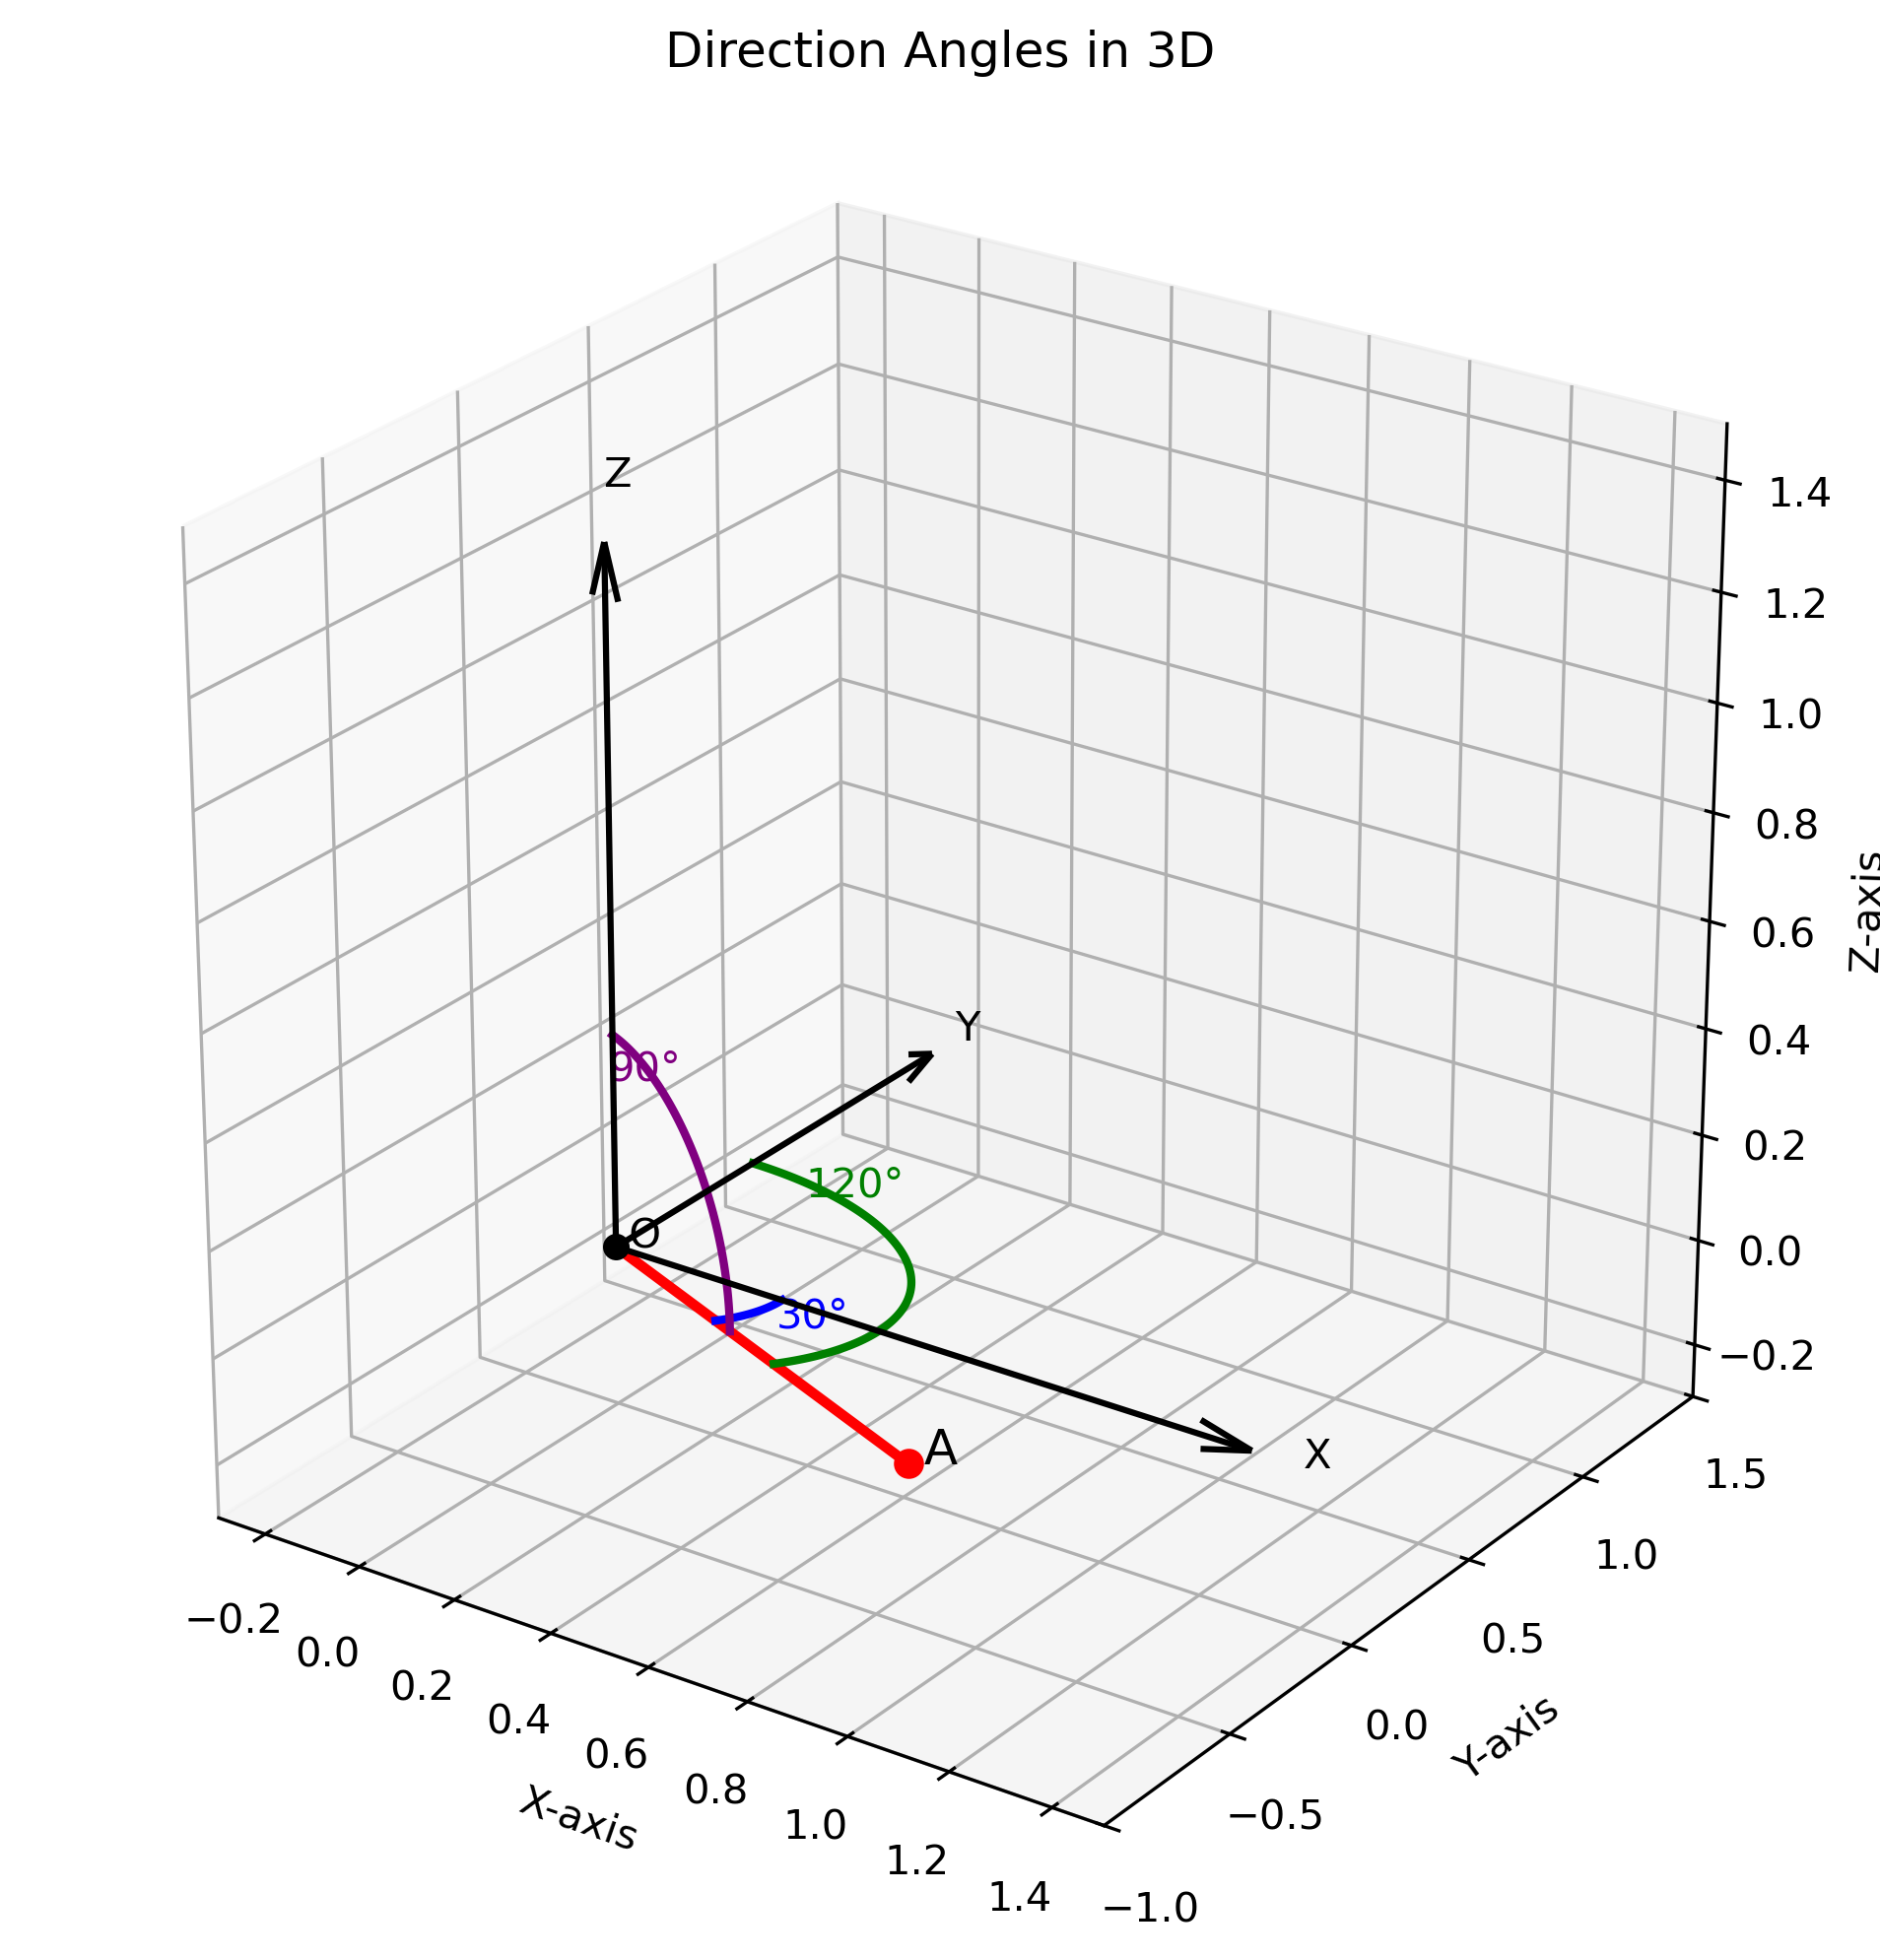
\includegraphics[
                width=0.5\textwidth,
                keepaspectratio
            ]{figs/s1218.png}
        };
    \end{tikzpicture}

\end{figure}


\item
ASSERTION : For any symmetric matrix $A$,
$B'AB$ is a skew-symmetric matrix.
\\REASON : A square matrix $P$ is skew-symmetric
if $P'=-P$.

Choose the correct option:

\begin{enumerate}
    \item Both Assertion and Reason are true,
    and Reason is the correct explanation of Assertion.
    \item Both Assertion and Reason are true,
    but Reason is not the correct explanation of Assertion .
    \item Assertion is true, but Reason is false.
    \item Assertion is false, but Reason is true.
\end{enumerate}

\solution
{Step 1: Check Assertion}
Given that $A$ is a symmetric matrix,
\begin{align}
A'=A.
\end{align}
Let
\begin{align}
P=B'AB.
\end{align}
Taking the transpose of $P$, we get
\begin{align}
P'=\brak{B'AB}'.
\end{align}
Using the transpose property $\brak{XYZ}'=Z'Y'X'$,
\begin{align}
P'=B'A'B.
\end{align}
Since $A'=A$,
\begin{align}
P'=B'AB.
\end{align}
Therefore,
\begin{align}
P'=P.
\end{align}
Hence, $B'AB$ is symmetric, not necessarily
skew-symmetric.
Thus, {Assertion  is false}. 

{Step 2: Check Reason}.
A square matrix $P$ is skew-symmetric if
\begin{align}
P'=-P.
\end{align}
This is the correct definition of a skew-symmetric matrix.
Therefore, {Reason  is true}.

Assertion is false, but Reason is true.

\item
ASSERTION : For two non-zero vectors
$\vec{a}$ and $\vec{b}$,
\begin{align}
\vec{a}\cdot\vec{b}=\vec{b}\cdot\vec{a}.
\end{align}

REASON : For two non-zero vectors
$\vec{a}$ and $\vec{b}$,
\begin{align}
\vec{a}\times\vec{b}=\vec{b}\times\vec{a}.
\end{align}

Choose the correct option:

\begin{enumerate}
    \item Both Assertion and Reason  are true,
    and Reason  is the correct explanation of Assertion .
    \item Both Assertion  and Reason are true,
    but Reason \brak{R} is not the correct explanation of Assertion .
    \item Assertion is true, but Reason is false.
    \item Assertion is false, but Reason is true.
\end{enumerate}

\solution
{Step 1: Verify Assertion }

The dot product of two vectors is commutative.

Using the formula \eqref{eq:EE26BTECH11211_Prob_1}
\begin{align}
\vec{a}\cdot\vec{b}
=|\vec{a}||\vec{b}|\cos\theta,
\end{align}
where $\theta$ is the angle between the vectors, we get
\begin{align}
\vec{b}\cdot\vec{a}
=|\vec{b}||\vec{a}|\cos\theta.
\end{align}
Since multiplication of real numbers is commutative,
\begin{align}
\vec{a}\cdot\vec{b}
=\vec{b}\cdot\vec{a}.
\end{align}
Therefore, {Assertion  is true}.

{Step 2: Verify Reason }

The cross product of two vectors is anti-commutative:
\begin{align}
\vec{a}\times\vec{b}
=-\brak{\vec{b}\times\vec{a}}.
\end{align}
In general, therefore,
\begin{align}
\vec{a}\times\vec{b}
\ne \vec{b}\times\vec{a}.
\end{align}
Hence,{Reason  is false}.
\\Assertion is true, but Reason is false.

\item
Find the value of
\begin{align}
\tan^{-1}\brak{-\frac{1}{\sqrt{3}}}
+\cot^{-1}\brak{\frac{1}{\sqrt{3}}}
+\tan^{-1}\sbrak{\sin\brak{-\frac{\pi}{2}}}.\label{eq:EE26BTECH11211_Prob_21.1}
\end{align}

\solution
We know that
\begin{align}
\tan^{-1}\left(-\frac{1}{\sqrt{3}}\right)
=-\frac{\pi}{6}.
\end{align}
Also, using the principal value of the inverse cotangent,
\begin{align}
\cot^{-1}\left(\frac{1}{\sqrt{3}}\right)
=\frac{\pi}{3}.
\end{align}
Since
\begin{align}
\sin\left(-\frac{\pi}{2}\right)=-1,
\end{align}
we have
\begin{align}
\tan^{-1}\sbrak{\sin\brak{-\frac{\pi}{2}}}
=\tan^{-1}\brak{-1}
=-\frac{\pi}{4}.
\end{align}
Substituting these values in \eqref{eq:EE26BTECH11211_Prob_21.1}, the given expression becomes
\begin{align}
 = -\frac{\pi}{6}+\frac{\pi}{3}-\frac{\pi}{4}.
\end{align}
Taking the LCM of $6$, $3$, and $4$, we obtain
\begin{align}
&-\frac{2\pi}{12}+\frac{4\pi}{12}-\frac{3\pi}{12}\\[4pt]
&=\frac{\brak{-2+4-3}\pi}{12}\\[4pt]
&=-\frac{\pi}{12}.
\end{align}

\item
Find the domain and range of the function
\begin{align}
f\brak{x}=\sin^{-1}\brak{x^2-4}.
\end{align}

\solution
{Step 1: Find the domain}

For $\sin^{-1}\brak{u}$ to be defined for real values,
\begin{align}
-1\leq u\leq 1.
\end{align}
Here, $u=x^2-4$. Therefore,
\begin{align}
-1\leq x^2-4\leq 1.
\end{align}
Adding $4$ throughout, we get
\begin{align}
3\leq x^2\leq 5.
\end{align}
Taking square roots and considering both positive
and negative values of $x$,
\begin{align}
\sqrt{3}\leq |x|\leq\sqrt{5}.
\end{align}
Hence,
\begin{align}
-\sqrt{5}\leq x\leq-\sqrt{3}
\end{align}
or
\begin{align}
\sqrt{3}\leq x\leq\sqrt{5}.
\end{align}
Therefore, the domain is
\begin{align}
[-\sqrt{5},-\sqrt{3}]
\cup[\sqrt{3},\sqrt{5}].
\end{align}
{Step 2: Find the range}

From the domain condition,
\begin{align}
3\leq x^2\leq 5.
\end{align}
Subtracting $4$,
\begin{align}
-1\leq x^2-4\leq 1.
\end{align}
Thus, the expression $x^2-4$ takes every value
in the interval $[-1,1]$.

Since
\begin{align}
f\brak{x}=\sin^{-1}\brak{x^2-4},
\end{align}
and the principal range of $\sin^{-1}\brak{u}$ is
\begin{align}
-\frac{\pi}{2}\leq\sin^{-1}\brak{u}\leq\frac{\pi}{2},
\end{align}
the range of $f\brak{x}$ is
\begin{align}
\left[-\frac{\pi}{2},\frac{\pi}{2}\right].
\end{align}
Final Answer
\begin{align}
\text{Domain}
=[-\sqrt{5},-\sqrt{3}]
\cup[\sqrt{3},\sqrt{5}]
\end{align}
\begin{align}
\text{Range}
=\left[-\frac{\pi}{2},\frac{\pi}{2}\right]
\end{align}

\item
If $f\brak{x}=\abs{\tan 2x}$,then find the value of $f'\brak{x}$ at $x=\dfrac{\pi}{3}$.

\solution
Given,
\begin{align}
f\brak{x}=|\tan 2x|.
\end{align}
At $x=\dfrac{\pi}{3}$,
\begin{align}
\tan 2x=\tan\left(\frac{2\pi}{3}\right)
=-\sqrt{3}<0.
\end{align}
Since $\tan 2x$ is negative near $x=\dfrac{\pi}{3}$,
\begin{align}
f\brak{x}=-\tan 2x.
\end{align}
Differentiating with respect to $x$,
\begin{align}
f'\brak{x}=-2\sec^2 2x.
\end{align}
Substituting $x=\dfrac{\pi}{3}$,
\begin{align}
f'\left(\frac{\pi}{3}\right)
=-2\sec^2\left(\frac{2\pi}{3}\right).
\end{align}
We know that
\begin{align}
\cos\left(\frac{2\pi}{3}\right)=-\frac{1}{2}.
\end{align}
Therefore,
\begin{align}
\sec^2\left(\frac{2\pi}{3}\right)
=\frac{1}{\cos^2\brak{2\pi/3}}
=\frac{1}{1/4}=4.
\end{align}
Hence,
\begin{align}
f'\left(\frac{\pi}{3}\right)=-2\brak{4}=-8.
\end{align}

\begin{align}
f'\left(\frac{\pi}{3}\right)=-8
\end{align}

\item
If $y = cosec \brak{ cot^{-1}x}$, then prove that $\brak{1+x^2}\dfrac{dy}{dx}-xy=0$.

\solution
Given, $y=cosec\brak{cot^{-1}x}.$

Let
\begin{align}
\theta=cot^{-1}x.
\end{align}
Then
\begin{align}
cot\theta=x.
\end{align}
Using the identity
\begin{align}
cosec^2 \theta=1+cot^2 \theta,
\end{align}
we get
\begin{align}
cosec^2\theta=1+x^2.
\end{align}
Since $\theta = cot^{-1}x$ lies in $\brak{0,\pi}$,
$ cosec \theta $ is positive. Therefore,
\begin{align}
y=\sqrt{1+x^2}.
\end{align}
Squaring both sides,
\begin{align}
y^2=1+x^2.
\end{align}
Differentiating with respect to $x$,
\begin{align}
2y\frac{dy}{dx}=2x.
\end{align}
Thus,
\begin{align}
\frac{dy}{dx}=\frac{x}{y}.
\end{align}
Multiplying both sides by $\brak{1+x^2}$,
\begin{align}
\brak{1+x^2}\frac{dy}{dx}
=\brak{1+x^2}\frac{x}{y}.
\end{align}
Since $y^2=1+x^2$,
\begin{align}
\brak{1+x^2}\frac{dy}{dx}
=\frac{y^2x}{y}=xy.
\end{align}
Therefore,
\begin{align}
\brak{1+x^2}\frac{dy}{dx}-xy=xy-xy=0.
\end{align}
Hence proved.



\item
If $M$ and $m$ denote the local maximum and local minimum
values of the function $f\brak{x}=x+\dfrac{1}{x}, \qquad x\ne 0,$
respectively, find the value of $\brak{M-m}$.

\solution
Given,
\begin{align}
f\brak{x}=x+\frac{1}{x}.
\end{align}
{Step 1: Find the first derivative}

Differentiating with respect to $x$,
\begin{align}
f'\brak{x}=1-\frac{1}{x^2}.
\end{align}
At the critical points,
\begin{align}
f'\brak{x}=0.
\end{align}
Therefore,
\begin{align}
1-\frac{1}{x^2}=0.
\end{align}
Multiplying by $x^2$, we get
\begin{align}
x^2-1=0.
\end{align}
Hence,
\begin{align}
\brak{x-1}\brak{x+1}=0.
\end{align}
Thus, the critical points are
\begin{align}
x=1 \quad \text{or} \quad x=-1.
\end{align}
{Step 2: Find the second derivative}

Differentiating again,
\begin{align}
f''\brak{x}=\frac{2}{x^3}.
\end{align}
At $x=-1$,
\begin{align}
f''\brak{-1}=\frac{2}{\brak{-1}^3}=-2<0.
\end{align}
Therefore, $f\brak{x}$ has a local maximum at $x=-1$.
\\The local maximum value is
\begin{align}
M=f\brak{-1}=-1+\frac{1}{-1}=-2.
\end{align}
At $x=1$,
\begin{align}
f''\brak{1}=\frac{2}{1^3}=2>0.
\end{align}
Therefore, $f\brak{x}$ has a local minimum at $x=1$.
\\The local minimum value is
\begin{align}
m=f\brak{1}=1+\frac{1}{1}=2.
\end{align}
{Step 3: Calculate $\brak{M-m}$}
\\Substituting $M=-2$ and $m=2$,
\begin{align}
M-m=-2-2.
\end{align}
Therefore,
\begin{align}
M-m=-4.
\end{align}

The following code gives the figure
\begin{lstlisting}[frame=single, basicstyle=\rmfamily, escapeinside={(*@}{@*)}]
(*@\makebox[\dimexpr\linewidth-2\fboxsep-2\fboxrule\relax][c]{codes/s1225.py}@*)
\end{lstlisting}
\begin{figure}[ht]
    \centering

    \begin{tikzpicture}
        \node[inner sep=0pt] at (0,0)
        {
            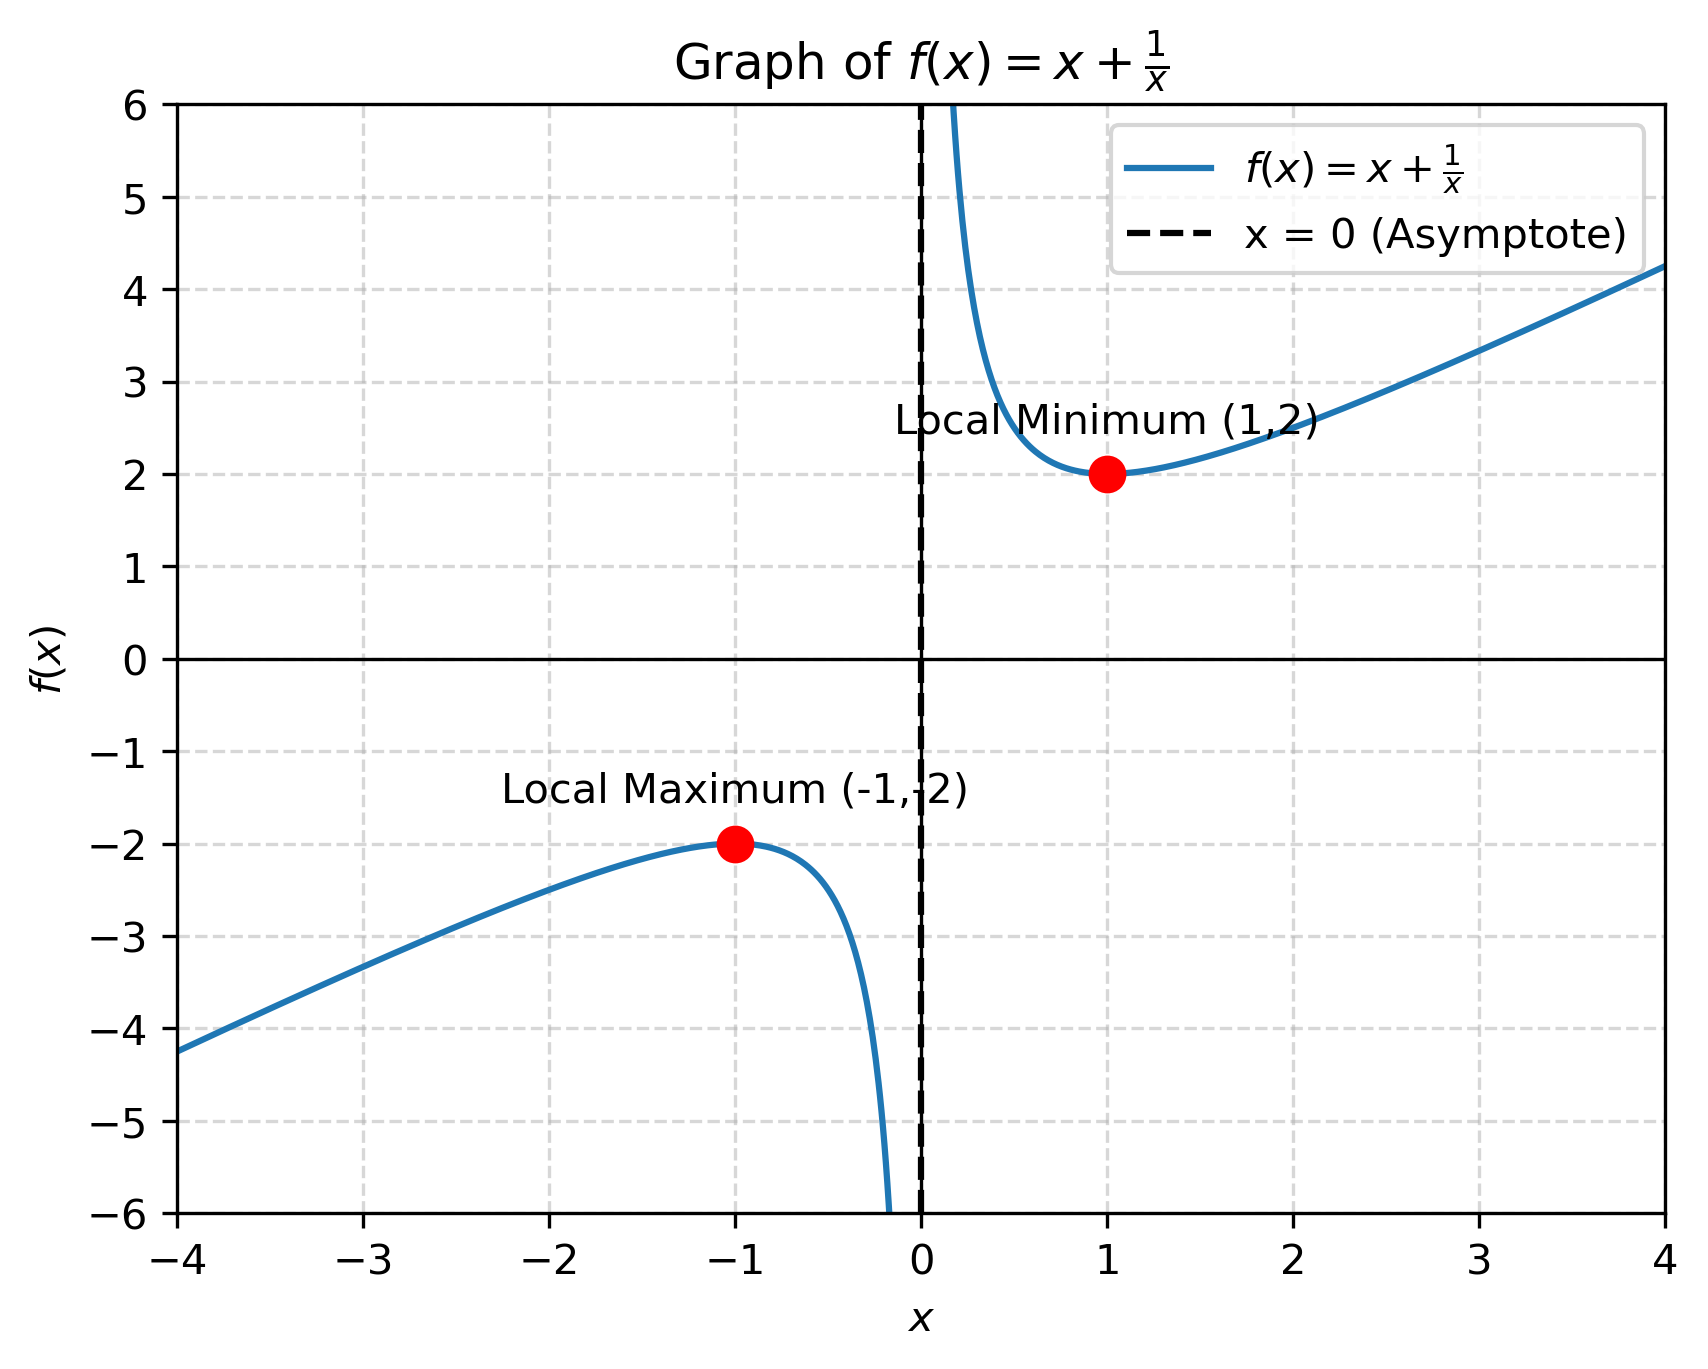
\includegraphics[
                width=0.5\textwidth,
                keepaspectratio
            ]{figs/s1225.png}
        };
    \end{tikzpicture}

\end{figure}

\item
Evaluate:
\begin{align}
I=\int \frac{e^{4x}-1}{e^{4x}+1}\,dx
\end{align}

\solution
Rewrite the integrand as
\begin{align}
I=\int\left(1-\frac{2}{e^{4x}+1}\right)\,dx.
\end{align}
Therefore,
\begin{align}
I=x-2\int\frac{1}{e^{4x}+1}\,dx.
\end{align}
Multiply the numerator and denominator of the
integrand by $e^{-4x}$:
\begin{align}
I=x-2\int\frac{e^{-4x}}{1+e^{-4x}}\,dx.\label{eq:EE26BTECH11211_Prob_26.4}
\end{align}
Let
\begin{align}
u=1+e^{-4x}.
\end{align}
Then
\begin{align}
du=-4e^{-4x}\,dx.
\end{align}
Hence by substituting \eqref{eq:EE26BTECH11211_Prob_26.4} becomes ,
\begin{align}
I
&=x-2\left(-\frac14\int\frac{du}{u}\right)\\[6pt]
\end{align}
by using \eqref{eq:EE26BTECH11211_Prob_4.3}
\begin{align}
I=x+\frac12\ln|u|+C.
\end{align}
Substituting $u=1+e^{-4x}$,
\begin{align}
I=x+\frac12\ln\brak{1+e^{-4x}}+C.
\end{align}
Using
\begin{align}
1+e^{-4x}=\frac{e^{4x}+1}{e^{4x}},
\end{align}
we obtain
\begin{align}
I
&=x+\frac12\ln\left(
\frac{e^{4x}+1}{e^{4x}}
\right)+C\\[6pt]
&=x+\frac12\ln\brak{e^{4x}+1}-2x+C\\[6pt]
&=\frac12\ln\brak{e^{4x}+1}-x+C.
\end{align}

\item
Show that $f\brak{x}=e^x-e^{-x}+x-\tan^{-1}x$ is strictly increasing in its domain.

\solution
Given,
\begin{align}
f\brak{x}=e^x-e^{-x}+x-\tan^{-1}x.
\end{align}
The domain of the function is $\mathbb{R}.$

{Step 1: Differentiate the function}

Differentiating with respect to $x$, we get
\begin{align}
f'\brak{x}=e^x+e^{-x}+1-\frac{1}{1+x^2}.
\end{align}
Rearranging,
\begin{align}
f'\brak{x}=e^x+e^{-x}
+\left(1-\frac{1}{1+x^2}\right).
\end{align}
Simplifying the expression in parentheses,
\begin{align}
f'\brak{x}=e^x+e^{-x}+\frac{x^2}{1+x^2}.
\end{align}
{Step 2: Prove that $f'\brak{x}>0$}

We know that, for every real number $x$,
\begin{align}
e^x+e^{-x}= 2.
\end{align}
Also, since $x^2= 0$,
\begin{align}
\frac{x^2}{1+x^2}= 0.
\end{align}
Therefore,
\begin{align}
f'\brak{x}=e^x+e^{-x}+\frac{x^2}{1+x^2}
= 2.
\end{align}
Hence,
\begin{align}
f'\brak{x}= 2>0
\qquad \forall x\in\mathbb{R}.
\end{align}
{Step 3: Conclusion}

Since
\begin{align}
f'\brak{x}>0
\qquad \forall x\in\mathbb{R},
\end{align}
the function $f\brak{x}$ is strictly increasing throughout
its domain.
\
The following code gives the figure
\begin{lstlisting}[frame=single, basicstyle=\rmfamily, escapeinside={(*@}{@*)}]
(*@\makebox[\dimexpr\linewidth-2\fboxsep-2\fboxrule\relax][c]{codes/s1227.py}@*)
\end{lstlisting}
\begin{figure}[ht]
    \centering

    \begin{tikzpicture}
        \node[inner sep=0pt] at (0,0)
        {
            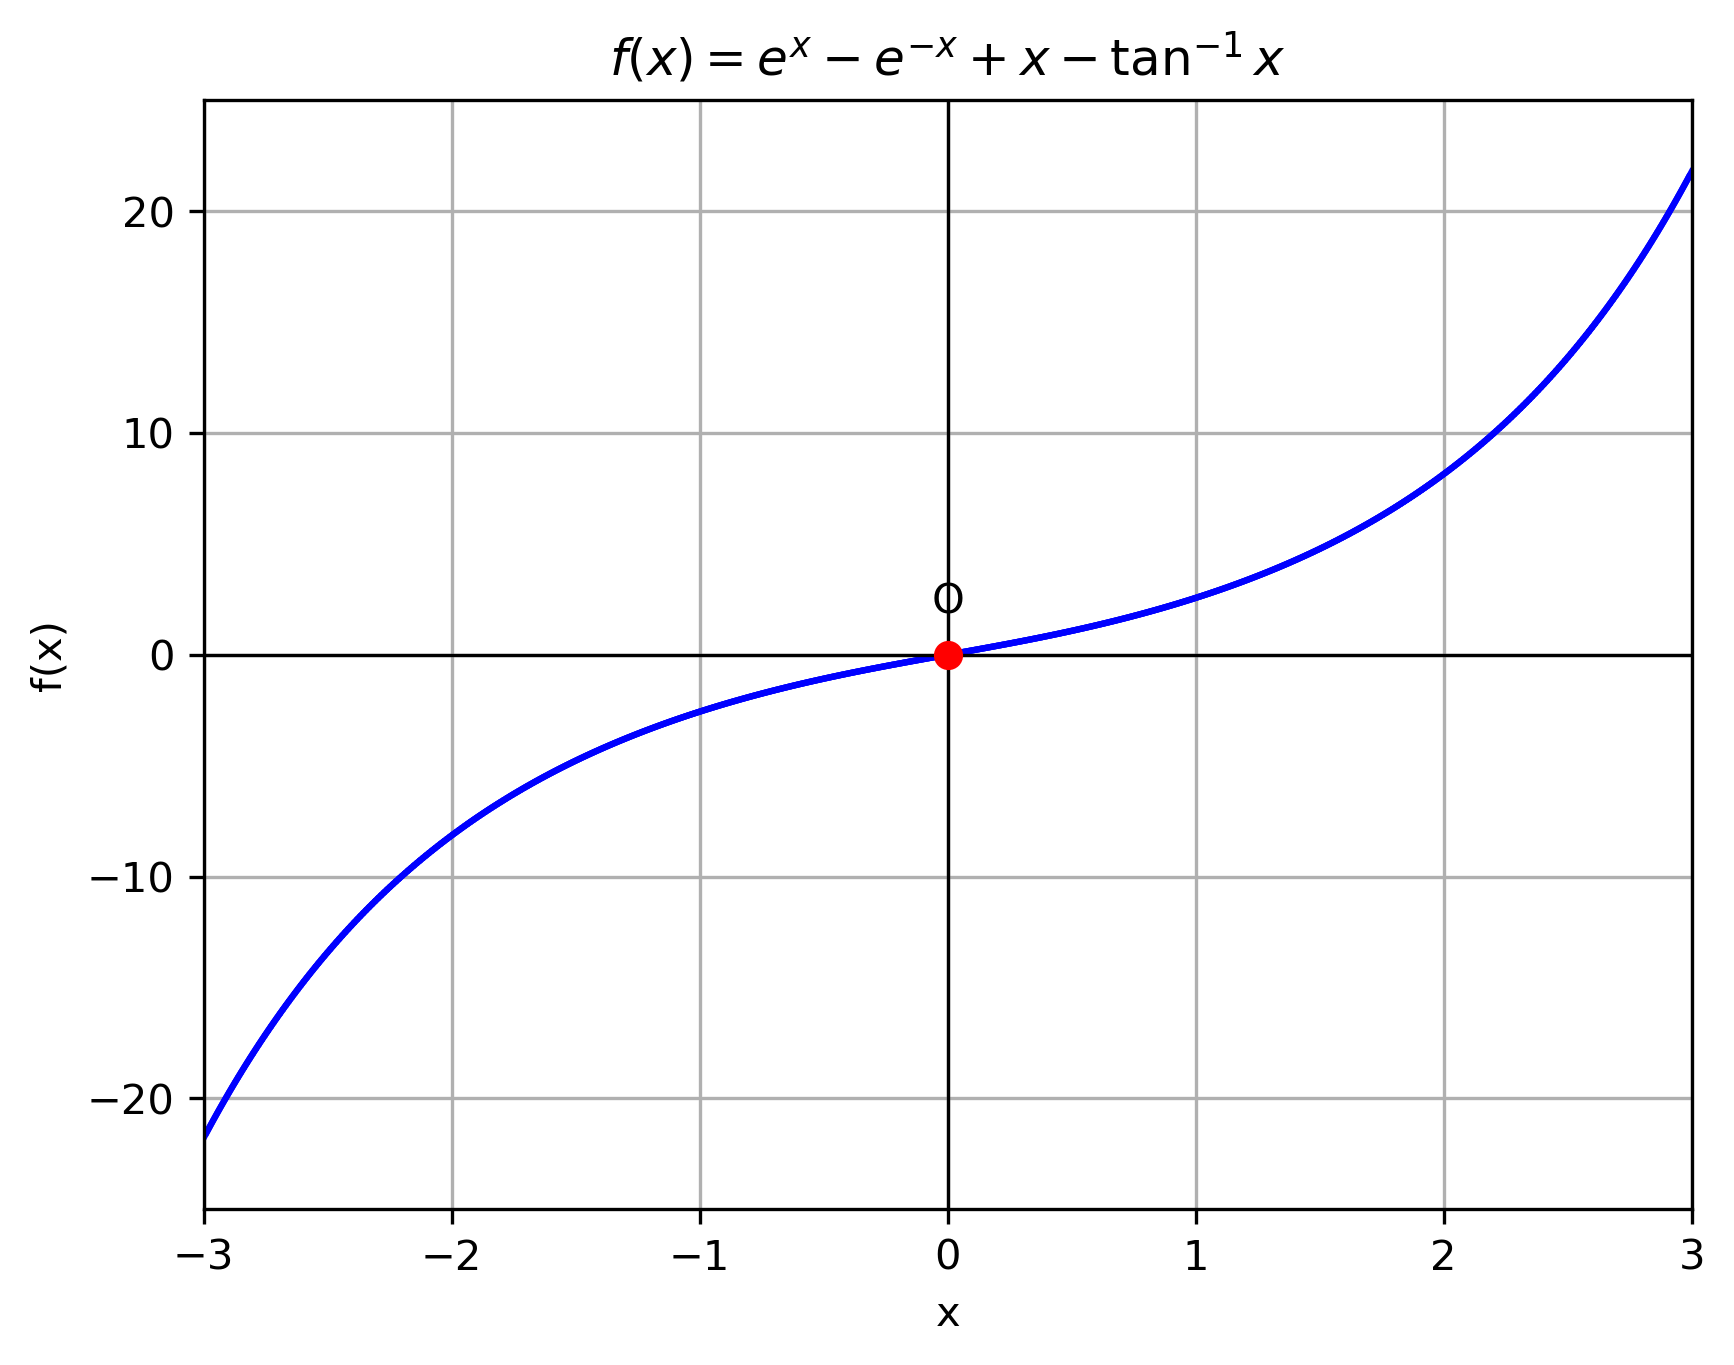
\includegraphics[
                width=0.5\textwidth,
                keepaspectratio
            ]{figs/s1227.png}
        };
    \end{tikzpicture}

\end{figure}

\item
If
$
x=e^{\cos 3t}
\qquad \text{and} \qquad
y=e^{\sin 3t},
$
prove that
$
\frac{dy}{dx}
=-\frac{y\log x}{x\log y}.
$

\solution
Given,
\begin{align}
x=e^{\cos 3t}
 \qquad \text{and} \qquad
y=e^{\sin 3t}.
\end{align}
Taking logarithms on both sides, we get
\begin{align}
\log x=\cos 3t
\end{align}
and
\begin{align}
\log y=\sin 3t.
\end{align}
{Step 1: Differentiate $x$ with respect to $t$}
\\Given,
\begin{align}
x=e^{\cos 3t}.
\end{align}
Differentiating with respect to $t$ using the formulae \eqref{eq:EE26BTECH11211_Prob_13},
\begin{align}
\frac{dx}{dt}
=e^{\cos 3t}\brak{-3\sin 3t}.
\end{align}
Since $x=e^{\cos 3t}$ and $\sin 3t=\log y$,
\begin{align}
\frac{dx}{dt}=-3x\log y.
\end{align}
{Step 2: Differentiate $y$ with respect to $t$ using the }
\\Given,
\begin{align}
y=e^{\sin 3t}.
\end{align}
Differentiating with respect to $t$ using the formulae \eqref{eq:EE26BTECH11211_Prob_13},,
\begin{align}
\frac{dy}{dt}
=e^{\sin 3t}\brak{3\cos 3t}.
\end{align}
Since $y=e^{\sin 3t}$ and $\cos 3t=\log x$,
\begin{align}
\frac{dy}{dt}=3y\log x.
\end{align}
{Step 3: Calculate $\dfrac{dy}{dx}$}
\\Using the formula for parametric differentiation,
\begin{align}
\frac{dy}{dx}
=\frac{\dfrac{dy}{dt}}{\dfrac{dx}{dt}}.
\end{align}
Substituting the values obtained above,
\begin{align}
\frac{dy}{dx}
=\frac{3y\log x}{-3x\log y}.
\end{align}
Cancelling $3$, we get
\begin{align}
\frac{dy}{dx}
=-\frac{y\log x}{x\log y}.
\end{align}
Hence proved.

\item
Show that
\begin{align}
\frac{d}{dx}\brak{|x|}=\frac{|x|}{x},
\qquad x\ne 0.
\end{align}

\solution
We know that the modulus function is defined as
\begin{align}
|x|=
\begin{cases}
x, & x>0,\\
-x, & x<0.
\end{cases}
\end{align}
{Case 1: When $x>0$}
\\Since $|x|=x$,
\begin{align}
\frac{d}{dx}\brak{|x|}
=\frac{d}{dx}\brak{x}=1.
\end{align}
Also, for $x>0$,
\begin{align}
\frac{|x|}{x}=\frac{x}{x}=1.
\end{align}
Therefore,
\begin{align}
\frac{d}{dx}\brak{|x|}=\frac{|x|}{x}.
\end{align}
{Case 2: When $x<0$}
\\Since $|x|=-x$,
\begin{align}
\frac{d}{dx}\brak{|x|}
=\frac{d}{dx}\brak{-x}=-1.
\end{align}
Also, for $x<0$,
\begin{align}
\frac{|x|}{x}=\frac{-x}{x}=-1.
\end{align}
Therefore,
\begin{align}
\frac{d}{dx}\brak{|x|}=\frac{|x|}{x}.
\end{align}
Thus, in both cases,
\begin{align}
\frac{d}{dx}\brak{|x|}=\frac{|x|}{x},
\qquad x\ne 0.
\end{align}
Hence proved.

\item
Evaluate:
\begin{align}
I=\int_{-2}^{2}\sqrt{\frac{2+x}{2-x}}\,dx
\end{align}

\solution
Let
\begin{align}
x=2\cos\theta.
\end{align}
Then,
\begin{align}
dx=-2\sin\theta\,d\theta.
\end{align}
Also,
\begin{align}
\sqrt{\frac{2+x}{2-x}}
=\sqrt{\frac{2+2\cos\theta}{2-2\cos\theta}}.
\end{align}
Using the identities
\begin{align}
1+\cos\theta=2\cos^2\frac{\theta}{2}
\end{align}
and
\begin{align}
1-\cos\theta=2\sin^2\frac{\theta}{2},
\end{align}
we obtain
\begin{align}
\sqrt{\frac{2+x}{2-x}}
=\cot\frac{\theta}{2}.
\end{align}
{Changing the limits:}
\\When $x=-2$,
\begin{align}
-2=2\cos\theta
\implies \theta=\pi.
\end{align}
When $x=2$,
\begin{align}
2=2\cos\theta
\implies \theta=0.
\end{align}
Therefore,
\begin{align}
I=\int_{\pi}^{0}
\cot\frac{\theta}{2}\brak{-2\sin\theta}\,d\theta.
\end{align}
Reversing the limits,
\begin{align}
I=2\int_0^\pi
\cot\frac{\theta}{2}\sin\theta\,d\theta.
\end{align}
Using
\begin{align}
\sin\theta
=2\sin\frac{\theta}{2}\cos\frac{\theta}{2},
\end{align}
we get
\begin{align}
I=4\int_0^\pi
\cos^2\frac{\theta}{2}\,d\theta.
\end{align}
Now, using
\begin{align}
\cos^2\frac{\theta}{2}
=\frac{1+\cos\theta}{2},
\end{align}
we obtain
\begin{align}
I=4\int_0^\pi\frac{1+\cos\theta}{2}\,d\theta.
\end{align}
Hence,
\begin{align}
I=2\int_0^\pi\brak{1+\cos\theta}\,d\theta.
\end{align}
Integrating,
\begin{align}
I=2\left[\theta+\sin\theta\right]_0^\pi.
\end{align}
Substituting the limits,
\begin{align}
I=2\left[\brak{\pi+0}-\brak{0+0}\right].
\end{align}
Thus,
\begin{align}
I=2\pi
\end{align}

\item
Evaluate:
\begin{align}
I=\int\frac{1}{x\left[\brak{\log x}^2-3\log x-4\right]}\,dx.
\end{align}
\solution
\\Let
\begin{align}
t=\log x.
\end{align}
Then,
\begin{align}
dt=\frac{1}{x}\,dx.
\end{align}
Therefore,
\begin{align}
I=\int\frac{1}{t^2-3t-4}\,dt.
\end{align}
Factorising the denominator,
\begin{align}
t^2-3t-4=\brak{t-4}\brak{t+1}.
\end{align}
Hence,
\begin{align}
I=\int\frac{1}{\brak{t-4}\brak{t+1}}\,dt.
\end{align}
Using partial fractions, let
\begin{align}
\frac{1}{\brak{t-4}\brak{t+1}}
=\frac{A}{t-4}+\frac{B}{t+1}.\label{eq:EE26BTECH11211_Prob_31.7}
\end{align}
Multiplying both sides by $\brak{t-4}\brak{t+1}$,
\begin{align}
1=A\brak{t+1}+B\brak{t-4}.
\end{align}
Putting $t=4$,
\begin{align}
1=5A
\implies A=\frac{1}{5}.
\end{align}
Putting $t=-1$,
\begin{align}
1=-5B
\implies B=-\frac{1}{5}.
\end{align}
Therefore substituting A nad B in \eqref{eq:EE26BTECH11211_Prob_31.7} we get,
\begin{align}
I=\frac{1}{5}\int\frac{1}{t-4}\,dt
-\frac{1}{5}\int\frac{1}{t+1}\,dt.
\end{align}
Integrating,
\begin{align}
I=\frac{1}{5}\log|t-4|
-\frac{1}{5}\log|t+1|+C.
\end{align}
Combining the logarithms,
\begin{align}
I=\frac{1}{5}\log\left|
\frac{t-4}{t+1}
\right|+C.
\end{align}
Substituting $t=\log x$, we obtain
\begin{align}
I=\frac{1}{5}\log\left|
\frac{\log x-4}{\log x+1}
\right|+C
\end{align}

\item
Find the particular solution of the differential equation
$2xy+y^2-2x^2\frac{dy}{dx}=0,$given that $y=2$ when $x=1$.

\solution
Rearranging the given equation,
\begin{align}
2x^2\frac{dy}{dx}=2xy+y^2.
\end{align}
Therefore,
\begin{align}
\frac{dy}{dx}=\frac{y}{x}+\frac{y^2}{2x^2}.
\end{align}
This is a homogeneous differential equation. Let
\begin{align}
y=vx,
\end{align}
where $v$ is a function of $x$.
\\Differentiating with respect to $x$,
\begin{align}
\frac{dy}{dx}=v+x\frac{dv}{dx}.
\end{align}
Substituting these expressions into the differential equation,
\begin{align}
v+x\frac{dv}{dx}=v+\frac{v^2}{2}.
\end{align}
Simplifying,
\begin{align}
x\frac{dv}{dx}=\frac{v^2}{2}.
\end{align}
Separating the variables,
\begin{align}
\frac{dv}{v^2}=\frac{dx}{2x}.
\end{align}
Integrating both sides,
\begin{align}
\int v^{-2}\,dv=\frac{1}{2}\int\frac{dx}{x}.
\end{align}
Hence,
\begin{align}
-\frac{1}{v}=\frac{1}{2}\log|x|+C.
\end{align}
Since $v=\dfrac{y}{x}$,
\begin{align}
-\frac{x}{y}=\frac{1}{2}\log|x|+C.
\end{align}
{Applying the given condition:}
\\When $x=1$, $y=2$. Substituting these values,
\begin{align}
-\frac{1}{2}=\frac{1}{2}\log 1+C.
\end{align}
Since $\log 1=0$,
\begin{align}
C=-\frac{1}{2}.
\end{align}
Therefore,
\begin{align}
-\frac{x}{y}=\frac{1}{2}\log|x|-\frac{1}{2}.
\end{align}
Multiplying both sides by $-2$,
\begin{align}
\frac{2x}{y}=1-\log|x|.
\end{align}
Thus, the particular solution is
\begin{align}
y=\frac{2x}{1-\log|x|}
\end{align}


\item
Find the general solution of the differential equation
\begin{align}
y\,dx=\brak{x+2y^2}\,dy
\end{align}

\solution
Dividing both sides by $dy$,
\begin{align}
y\frac{dx}{dy}=x+2y^2.
\end{align}
Dividing by $y$,
\begin{align}
\frac{dx}{dy}=\frac{x}{y}+2y.
\end{align}
Rearranging,
\begin{align}
\frac{dx}{dy}-\frac{x}{y}=2y.
\end{align}
we can solve this above linear differential equation using \eqref{eq:EE26BTECH11211_Prob_14}
\begin{align}
\frac{dx}{dy}+P\brak{y}x=Q\brak{y},
\end{align}
where
\begin{align}
P\brak{y}=-\frac{1}{y},
\qquad Q\brak{y}=2y.
\end{align}
{Step 1: Find the integrating factor.}
\\The integrating factor is
\begin{align}
\mathrm{I.F.}=e^{\int P\brak{y}\,dy}.
\end{align}
Therefore,
\begin{align}
\mathrm{I.F.}=e^{-\int\frac{1}{y}\,dy}
=e^{-\log|y|}
=\frac{1}{y}.
\end{align}
from  \eqref{eq:EE26BTECH11211_Prob_14}
\begin{align}
x\brak{\frac{1}{y}}=\int2y\frac{1}{y}\,dy
\end{align}
\begin{align}
x\brak{\frac{1}{y}}=2y+C
\end{align}

Thus, the general solution is
\begin{align}
x=2y^2+Cy,
\end{align}
where $C$ is an arbitrary constant.

\item
The position vectors of the vertices $A$, $B$ and $C$ of a triangle
$ABC$ are $\vec{A}=2\vec{i}-\vec{j}+\vec{k},\vec{B}=\vec{i}-3\vec{j}-5\vec{k}$,
and $\vec{C}=3\vec{i}-4\vec{j}-4\vec{k}$.
Find all the angles of triangle $ABC$.

\solution
The position vectors are
\begin{align}
A=\brak{2,-1,1},\quad B=\brak{1,-3,-5},\quad C=\brak{3,-4,-4}.
\end{align}
{Step 1: Find the vectors along the sides.}
\\We have
\begin{align}
\overrightarrow{AB}=\vec{B}-\vec{A}.
\end{align}
Therefore,
\begin{align}
\overrightarrow{AB}
=\brak{1-2}\vec{i}+\brak{-3+1}\vec{j}+\brak{-5-1}\vec{k}.
\end{align}
Hence,
\begin{align}
\overrightarrow{AB}=-\vec{i}-2\vec{j}-6\vec{k}.
\end{align}
Similarly,
\begin{align}
\overrightarrow{AC}=\vec{C}-\vec{A},
\end{align}
which gives
\begin{align}
\overrightarrow{AC}
=\vec{i}-3\vec{j}-5\vec{k}.
\end{align}
Also,
\begin{align}
\overrightarrow{BC}=\vec{C}-\vec{B},
\end{align}
so
\begin{align}
\overrightarrow{BC}=2\vec{i}-\vec{j}+\vec{k}.
\end{align}
{Step 2: Find angle $A$.}
\\The angle $A$ is the angle between
$\overrightarrow{AB}$ and $\overrightarrow{AC}$.
\\Using the dot product formula,
\begin{align}
\cos A=
\frac{\overrightarrow{AB}\cdot\overrightarrow{AC}}
{|\overrightarrow{AB}||\overrightarrow{AC}|}.
\end{align}
First, calculate the dot product:
\begin{align}
\overrightarrow{AB}\cdot\overrightarrow{AC}
=\brak{-1}\brak{1}+\brak{-2}\brak{-3}+\brak{-6}\brak{-5}.
\end{align}
Thus,
\begin{align}
\overrightarrow{AB}\cdot\overrightarrow{AC}
=-1+6+30=35.
\end{align}
The magnitudes are
\begin{align}
|\overrightarrow{AB}|
=\sqrt{\brak{-1}^2+\brak{-2}^2+\brak{-6}^2}
=\sqrt{41},
\end{align}
and
\begin{align}
|\overrightarrow{AC}|
=\sqrt{1^2+\brak{-3}^2+\brak{-5}^2}
=\sqrt{35}.
\end{align}
Therefore,
\begin{align}
\cos A=\frac{35}{\sqrt{41}\sqrt{35}}
=\sqrt{\frac{35}{41}}.
\end{align}
Hence,
\begin{align}
A=\cos^{-1}\sqrt{\frac{35}{41}}.
\end{align}
{Step 3: Find angle $B$.}
\\The angle $B$ is the angle between
$\overrightarrow{BA}$ and $\overrightarrow{BC}$.
We have
\begin{align}
\overrightarrow{BA}
=\vec{i}+2\vec{j}+6\vec{k}.
\end{align}
Using the dot product formula \eqref{eq:EE26BTECH11211-Prob_7.1},
\begin{align}
\cos B=
\frac{\overrightarrow{BA}\cdot\overrightarrow{BC}}
{|\overrightarrow{BA}||\overrightarrow{BC}|}.
\end{align}
Calculating the dot product,
\begin{align}
\overrightarrow{BA}\cdot\overrightarrow{BC}
=\brak{1}\brak{2}+\brak{2}\brak{-1}+\brak{6}\brak{1}.
\end{align}
Thus,
\begin{align}
\overrightarrow{BA}\cdot\overrightarrow{BC}
=2-2+6=6.
\end{align}
Also,
\begin{align}
|\overrightarrow{BA}|=\sqrt{41},
\end{align}
and
\begin{align}
|\overrightarrow{BC}|
=\sqrt{2^2+\brak{-1}^2+1^2}
=\sqrt{6}.
\end{align}
Therefore,
\begin{align}
\cos B=\frac{6}{\sqrt{41}\sqrt{6}}
=\sqrt{\frac{6}{41}}.
\end{align}
Hence,
\begin{align}
B=\cos^{-1}\sqrt{\frac{6}{41}}
\end{align}
{Step 4: Find angle $C$.}
\\The angle $C$ is the angle between
$\overrightarrow{CA}$ and $\overrightarrow{CB}$.
\\We have
\begin{align}
\overrightarrow{CA}
=-\vec{i}+3\vec{j}+5\vec{k},
\end{align}
and
\begin{align}
\overrightarrow{CB}
=-2\vec{i}+\vec{j}-\vec{k}.
\end{align}
Their dot product is
\begin{align}
\overrightarrow{CA}\cdot\overrightarrow{CB}
=\brak{-1}\brak{-2}+\brak{3}\brak{1}+\brak{5}\brak{-1}.
\end{align}
Therefore,
\begin{align}
\overrightarrow{CA}\cdot\overrightarrow{CB}
=2+3-5=0.
\end{align}
Since the dot product is zero, the vectors are perpendicular.
\\Hence,
\begin{align}
C=90^\circ
\end{align}
\textbf{Final Answer}\\
\\The three angles of triangle $ABC$ are
\begin{align}
A&=\cos^{-1}\sqrt{\frac{35}{41}},\\[4pt]
B&=\cos^{-1}\sqrt{\frac{6}{41}},\\[4pt]
C&=90^\circ.
\end{align}

\item
A pair of dice is thrown simultaneously. If $X$ denotes the absolute
difference of the  numbers appearing on top of the dice,then find the
probability distribution of $X$.

\solution
When two dice are thrown simultaneously, the total number of possible
outcomes is
\begin{align}
n\brak{S}=6\times 6=36.
\end{align}
Let the numbers appearing on the two dice be $a$ and $b$.
\\The random variable $X$ is defined as
\begin{align}
X=|a-b|.
\end{align}
Since the numbers on the dice range from $1$ to $6$, the possible
values of $X$ are
\begin{align}
X=0,1,2,3,4,5.
\end{align}
{Step 1: Calculate the number of outcomes for each value of $X$.}
\\{Case 1: $X=0$}
\\Both dice show the same number.
\\The outcomes are
\begin{align}
\brak{1,1},\brak{2,2},\brak{3,3},\brak{4,4},\brak{5,5},\brak{6,6}.
\end{align}
Therefore,
\begin{align}
P\brak{X=0}=\frac{6}{36}=\frac{1}{6}.
\end{align}
{Case 2: $X=1$}
\\The outcomes are
\begin{align}
&\brak{1,2},\brak{2,1},\brak{2,3},\brak{3,2},\\
&\brak{3,4},\brak{4,3},\brak{4,5},\brak{5,4},\\
&\brak{5,6},\brak{6,5}.
\end{align}
\\There are $10$ outcomes. Hence,
\begin{align}
P\brak{X=1}=\frac{10}{36}=\frac{5}{18}.
\end{align}
{Case 3: $X=2$}
\\There are $8$ outcomes:
\begin{align}
&\brak{1,3},\brak{3,1},\brak{2,4},\brak{4,2},\\
&\brak{3,5},\brak{5,3},\brak{4,6},\brak{6,4}.
\end{align}
Therefore,
\begin{align}
P\brak{X=2}=\frac{8}{36}=\frac{2}{9}.
\end{align}
{Case 4: $X=3$}
\\There are $6$ outcomes:
\begin{align}
\brak{1,4},\brak{4,1},\brak{2,5},\brak{5,2},\brak{3,6},\brak{6,3}.
\end{align}
Therefore,
\begin{align}
P\brak{X=3}=\frac{6}{36}=\frac{1}{6}.
\end{align}
{Case 5: $X=4$}
There are $4$ outcomes:
\begin{align}
\brak{1,5},\brak{5,1},\brak{2,6},\brak{6,2}.
\end{align}
Therefore,
\begin{align}
P\brak{X=4}=\frac{4}{36}=\frac{1}{9}.
\end{align}
{Case 6: $X=5$}
\\There are $2$ outcomes:
\begin{align}
\brak{1,6},\brak{6,1}.
\end{align}
Therefore,
\begin{align}
P\brak{X=5}=\frac{2}{36}=\frac{1}{18}.
\end{align}
{Step 2: Construct the probability distribution.}
\\The probability distribution of $X$ is given by
\begin{align}
\begin{array}{c|cccccc}
X & 0 & 1 & 2 & 3 & 4 & 5\\
\hline
P\brak{X} & \dfrac{1}{6} & \dfrac{5}{18} &
\dfrac{2}{9} & \dfrac{1}{6} &
\dfrac{1}{9} & \dfrac{1}{18}
\end{array}
\end{align}
{Verification:}
\\The sum of all probabilities must equal $1$.
\begin{align}
\sum P\brak{X}
&=\frac{1}{6}+\frac{5}{18}+\frac{2}{9}
+\frac{1}{6}+\frac{1}{9}+\frac{1}{18}\\[4pt]
&=\frac{3+5+4+3+2+1}{18}\\[4pt]
&=\frac{18}{18}\\[4pt]
&=1.
\end{align}
Hence, the probability distribution is correct.

\item
Evaluate:$I=\int x^2\sin^{-1}\brak{x^{3/2}}\,dx.$

\solution
Using integration by parts \eqref{eq:EE26BTECH11211_Prob_3.1},
\begin{align}
\int u\,dv=uv-\int v\,du.
\end{align}
Choose
\begin{align}
u=\sin^{-1}\brak{x^{3/2}},
\qquad dv=x^2\,dx.
\end{align}
Differentiating $u$ using the formulae \eqref{eq:EE26BTECH11211_Prob_15},
\begin{align}
du=\frac{1}{\sqrt{1-\brak{x^{3/2}}^2}}
\cdot\frac{3}{2}x^{1/2}\,dx.
\end{align}
Therefore,
\begin{align}
du=\frac{3\sqrt{x}}{2\sqrt{1-x^3}}\,dx.
\end{align}
Integrating $dv$,
\begin{align}
v=\int x^2\,dx=\frac{x^3}{3}.
\end{align}
Applying integration by parts,
\begin{align}
I=\frac{x^3}{3}\sin^{-1}\brak{x^{3/2}}
-\int\frac{x^3}{3}
\cdot\frac{3\sqrt{x}}{2\sqrt{1-x^3}}\,dx.
\end{align}
Simplifying,
\begin{align}
I=\frac{x^3}{3}\sin^{-1}\brak{x^{3/2}}
-\frac{1}{2}\int\frac{x^{7/2}}{\sqrt{1-x^3}}\,dx.
\end{align}
Let
\begin{align}
t=x^{3/2}.
\end{align}
Then
\begin{align}
dt=\frac{3}{2}\sqrt{x}\,dx,
\qquad
dx=\frac{2}{3\sqrt{x}}\,dt.
\end{align}
Since $x=t^{2/3}$, the remaining integral becomes
\begin{align}
\int\frac{x^{7/2}}{\sqrt{1-x^3}}\,dx
=\frac{2}{3}\int\frac{t^2}{\sqrt{1-t^2}}\,dt.
\end{align}
Using
\begin{align}
t=\sin\theta,
\qquad dt=\cos\theta\,d\theta,
\end{align}
we obtain
\begin{align}
\int\frac{t^2}{\sqrt{1-t^2}}\,dt
=\int\sin^2\theta\,d\theta.
\end{align}
Using the identity
\begin{align}
\sin^2\theta=\frac{1-\cos 2\theta}{2},
\end{align}
we get
\begin{align}
\int\sin^2\theta\,d\theta
=\frac{\theta}{2}-\frac{\sin 2\theta}{4}+C.
\end{align}
Substituting back,
\begin{align}
\int\frac{t^2}{\sqrt{1-t^2}}\,dt
=\frac{1}{2}\sin^{-1}t
-\frac{t\sqrt{1-t^2}}{2}+C.
\end{align}
Therefore,
\begin{align}
\int\frac{x^{7/2}}{\sqrt{1-x^3}}\,dx
=\frac{1}{3}\sin^{-1}\brak{x^{3/2}}
-\frac{x^{3/2}\sqrt{1-x^3}}{3}+C.
\end{align}
Substituting into the expression for $I$,
\begin{align}
I={}&\frac{x^3}{3}\sin^{-1}\brak{x^{3/2}}\\
&-\frac{1}{6}\sin^{-1}\brak{x^{3/2}}\\
&+\frac{x^{3/2}\sqrt{1-x^3}}{6}+C.
\end{align}
Hence, the final answer is
\begin{align}
I={}&\frac{x^3}{3}\sin^{-1}\brak{x^{3/2}}
-\frac{1}{6}\sin^{-1}\brak{x^{3/2}}\\
&+\frac{x^{3/2}\sqrt{1-x^3}}{6}+C.
\end{align}

\item
Show that the function $f:\mathbb{R}\to\mathbb{R}$ defined by $f\brak{x}=\frac{2x}{1+x^2}$
is neither one-one nor onto. Further, find a set $A$ so that the given function
$f:\mathbb{R}\to A$ becomes onto function.

\solution
The given function is
\begin{align}
f\brak{x}=\frac{2x}{1+x^2}.
\end{align}
{Step 1: Show that $f$ is not one-one.}
\\A function is one-one if distinct inputs always have distinct outputs.
\\Consider
\begin{align}
f\brak{2}=\frac{2\brak{2}}{1+2^2}
=\frac{4}{5}.
\end{align}
Also,
\begin{align}
f\left(\frac{1}{2}\right)
=\frac{2\left(\frac{1}{2}\right)}
{1+\left(\frac{1}{2}\right)^2}.
\end{align}
Simplifying,
\begin{align}
f\left(\frac{1}{2}\right)
=\frac{1}{1+\frac{1}{4}}
=\frac{4}{5}.
\end{align}
Therefore,
\begin{align}
f\brak{2}=f\left(\frac{1}{2}\right),
\end{align}
even though
\begin{align}
2\ne\frac{1}{2}.
\end{align}
Hence, $f$ is not one-one.
\begin{align}
f\text{ is not one-one.}
\end{align}
{Step 2: Show that $f$ is not onto $\mathbb{R}$.}
\\We have
\begin{align}
f\brak{x}=\frac{2x}{1+x^2}.
\end{align}
Since
\begin{align}
\brak{|x|-1}^2= 0,
\end{align}
we get
\begin{align}abel
x^2+1= 2|x|.
\end{align}
Therefore,
\begin{align}
\left|\frac{2x}{1+x^2}\right|\leq 1.
\end{align}
Thus,
\begin{align}
-1\leq f\brak{x}\leq 1.
\end{align}
Hence, the range of $f$ is contained in $[-1,1]$.
In fact, both endpoints are attained:
\begin{align}
f\brak{1}=1,\qquad f\brak{-1}=-1.
\end{align}
Therefore, the range is
\begin{align}
\operatorname{Range}\brak{f}=[-1,1].
\end{align}
Since the codomain is $\mathbb{R}$, values outside $[-1,1]$
are not attained. Hence, $f$ is not onto $\mathbb{R}$.
\begin{align}
f\text{ is not onto }\mathbb{R}.
\end{align}
{Step 3: Find the set $A$.}
\\For $f:\mathbb{R}\to A$ to be onto, its codomain must equal
its range.
Therefore,
\begin{align}
A=[-1,1].
\end{align}

Thus, $f:\mathbb{R}\to[-1,1]$ is onto.

\item
A relation $\mathbb{R}$ is defined on $\mathbb{N}\times\mathbb{N}$ $\brak{\text{where} \mathbb{N} \text{is the set of natural numbers}}$ as:
\begin{align}
\brak{a,b}\,R\,\brak{c,d}
\iff a-c=b-d.
\end{align}

Show that $R$ is an equivalence relation.

\solution
A relation is an equivalence relation if it is reflexive,
symmetric, and transitive.
\\We prove these three properties.
\\{Step 1: Reflexivity}
\\For any $\brak{a,b}\in\mathbb{N}\times\mathbb{N}$, we have
\begin{align}
a-a=0
\end{align}
and
\begin{align}
b-b=0.
\end{align}
Therefore,
\begin{align}
a-a=b-b.
\end{align}
By the definition of $R$,
\begin{align}
\brak{a,b}\,R\,\brak{a,b}.
\end{align}
Hence, $R$ is reflexive.
\begin{align}
R\text{ is reflexive.}
\end{align}

{Step 2: Symmetry}
\\Suppose
\begin{align}
\brak{a,b}\,R\,\brak{c,d}.
\end{align}
Then, by definition,
\begin{align}
a-c=b-d.
\end{align}
Multiplying both sides by $-1$, we obtain
\begin{align}
c-a=d-b.
\end{align}
Therefore,
\begin{align}
\brak{c,d}\,R\,\brak{a,b}.
\end{align}
Hence, $R$ is symmetric.
\begin{align}
R\text{ is symmetric.}
\end{align}
{Step 3: Transitivity}
\\Suppose
\begin{align}
\brak{a,b}\,R\,\brak{c,d}
\end{align}
and
\begin{align}
\brak{c,d}\,R\,\brak{e,f}.
\end{align}
Then,
\begin{align}
a-c=b-d
\end{align}
and
\begin{align}
c-e=d-f.
\end{align}
Adding these equations, we get
\begin{align}
\brak{a-c}+\brak{c-e}=\brak{b-d}+\brak{d-f}.
\end{align}
Simplifying,
\begin{align}
a-e=b-f.
\end{align}
Therefore,
\begin{align}
\brak{a,b}\,R\,\brak{e,f}.
\end{align}
Hence, $R$ is transitive.
\begin{align}
R\text{ is transitive.}
\end{align}
Since $R$ is reflexive, symmetric, and transitive, it follows that
\begin{align}
R\text{ is an equivalence relation.}
\end{align}

\item
Find the equation of the line which bisects the line segment joining
$A\brak{2,3,4}$ and $B\brak{4,5,8}$ and is perpendicular to the lines
$\dfrac{x-8}{3}=\dfrac{y+19}{-16}=\dfrac{z-10}{7}$ and $\dfrac{x-15}{3}=\dfrac{y-29}{8}=\dfrac{z+5}{-5}$.

\solution
The required line passes through the midpoint of $AB$ and is
perpendicular to both given lines.

{Step 1: Find the midpoint of $AB$.}

The coordinates of the midpoint $M$ of $AB$ are
\begin{align}
M=\left(
\frac{x_1+x_2}{2},
\frac{y_1+y_2}{2},
\frac{z_1+z_2}{2}
\right).
\end{align}
Substituting $A\brak{2,3,4}$ and $B\brak{4,5,8}$,
\begin{align}
M=\left(
\frac{2+4}{2},
\frac{3+5}{2},
\frac{4+8}{2}
\right).
\end{align}
Therefore,
\begin{align}
\boxed{M=\brak{3,4,6}}.
\end{align}
{Step 2: Find the direction vectors of the given lines.}
\\The first line is
\begin{align}
\frac{x-8}{3}=\frac{y+19}{-16}=\frac{z-10}{7}.
\end{align}
Its direction vector is
\begin{align}
\vec{d}_1=3\vec{i}-16\vec{j}+7\vec{k}.
\end{align}
Thus,
\begin{align}
\vec{d}_1=\brak{3,-16,7}.
\end{align}
The second line is
\begin{align}
\frac{x-15}{3}=\frac{y-29}{8}=\frac{z+5}{-5}.
\end{align}
Its direction vector is
\begin{align}
\vec{d}_2=3\vec{i}+8\vec{j}-5\vec{k}.
\end{align}
Thus,
\begin{align}
\vec{d}_2=\brak{3,8,-5}.
\end{align}
{Step 3: Find the direction vector of the required line.}
\\Since the required line is perpendicular to both given lines,
its direction vector must be perpendicular to both
$\vec{d}_1$ and $\vec{d}_2$.

Therefore, we take their cross product:
\begin{align}
\vec{d}=\vec{d}_1\times\vec{d}_2.
\end{align}
Expanding the determinant,
\begin{align}
\vec{d}=
\myvec{
\vec{i}&\vec{j}&\vec{k}\\
3&-16&7\\
3&8&-5
}.
\end{align}
Expanding along the first row,
\begin{align}
\vec{d}
={}&\vec{i}\big[\brak{-16}\brak{-5}-7\brak{8}\big]\\
&-\vec{j}\big[3\brak{-5}-7\brak{3}\big]\\
&+\vec{k}\big[3\brak{8}-\brak{-16}\brak{3}\big].
\end{align}
Simplifying,
\begin{align}
\vec{d}
&=24\vec{i}+36\vec{j}+72\vec{k}\\
&=12\brak{2\vec{i}+3\vec{j}+6\vec{k}}.
\end{align}
We may therefore take the direction vector as
\begin{align}
\vec{d}=\brak{2,3,6}
\end{align}
{Step 4: Write the equation of the required line.}
\\The line passes through $M\brak{3,4,6}$ and has direction vector
$\brak{2,3,6}$.
\\The symmetric equation of a line passing through
$\brak{x_1,y_1,z_1}$ with direction ratios $\brak{a,b,c}$ is
\begin{align}
\frac{x-x_1}{a}
=\frac{y-y_1}{b}
=\frac{z-z_1}{c}.
\end{align}
Substituting the midpoint and direction ratios, we obtain
\begin{align}
\frac{x-3}{2}
=\frac{y-4}{3}
=\frac{z-6}{6}
\end{align}
The following code gives the figure
\begin{lstlisting}[frame=single, basicstyle=\rmfamily, escapeinside={(*@}{@*)}]
(*@\makebox[\dimexpr\linewidth-2\fboxsep-2\fboxrule\relax][c]{codes/s1239.py}@*)
\end{lstlisting}
\begin{figure}[ht]
    \centering

    \begin{tikzpicture}
        \node[inner sep=0pt] at (0,0)
        {
            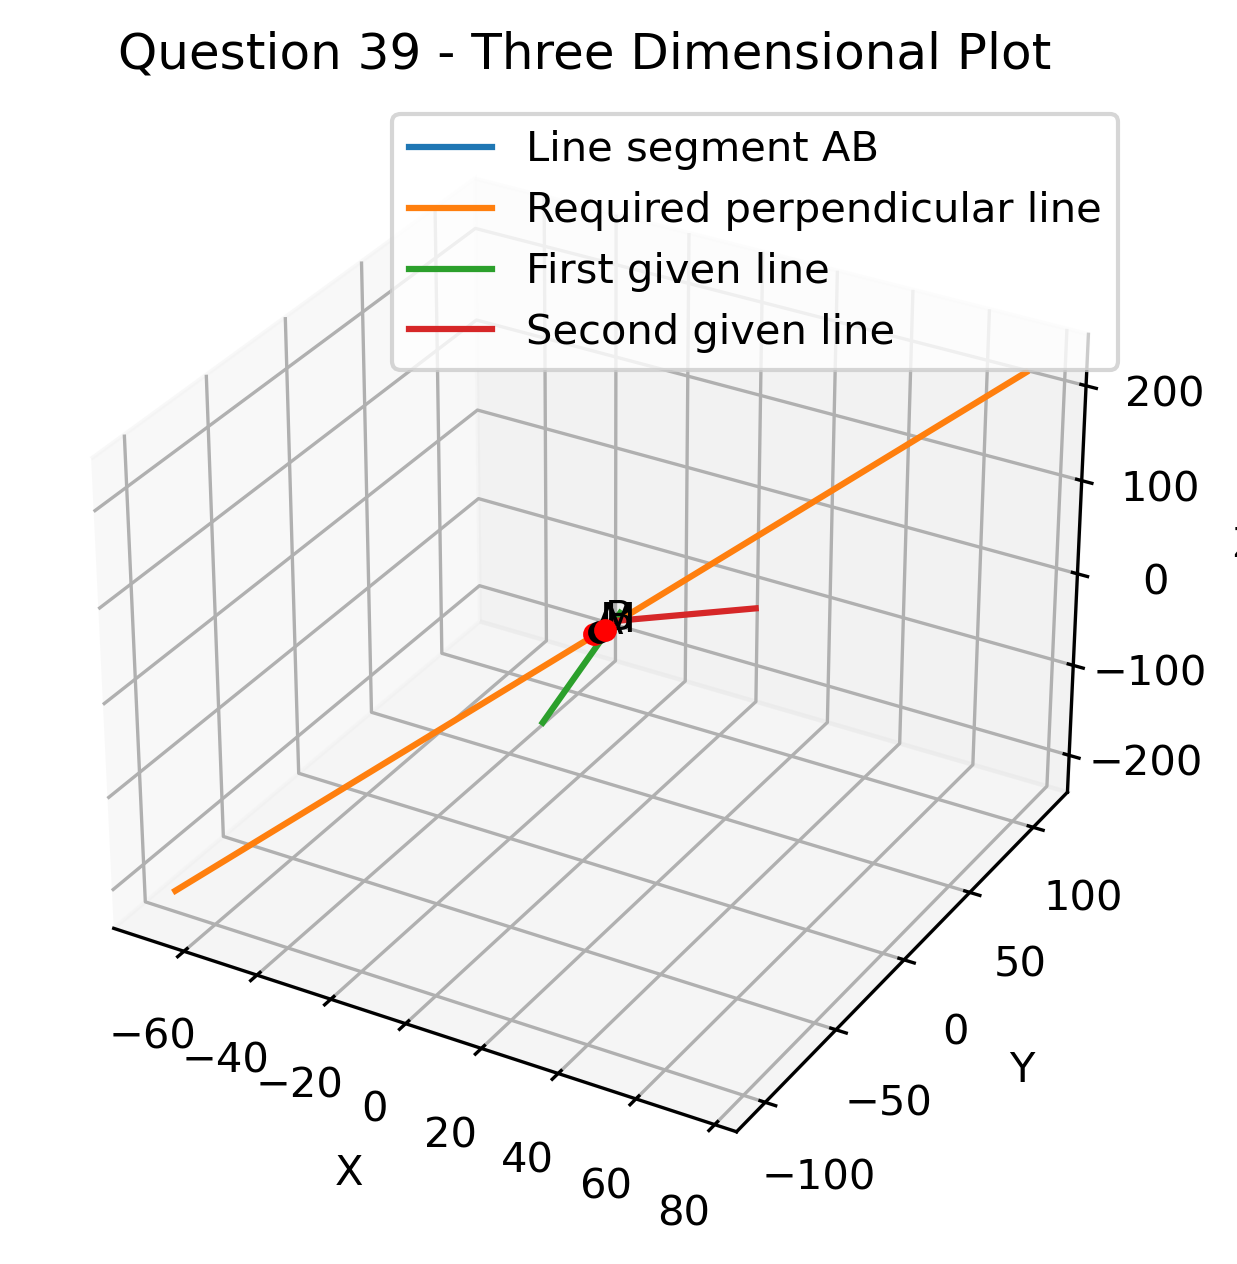
\includegraphics[
                width=0.5\textwidth,
                keepaspectratio
            ]{figs/s1239.png}
        };
    \end{tikzpicture}

\end{figure}

\item Solve the following system of equations using matrices.
\begin{align}
    \frac{2}{x}+\frac{3}{y}+\frac{10}{z}&=4\\
    \frac{4}{x}-\frac{6}{y}+\frac{5}{z}&=1\\
    \frac{6}{x}+\frac{9}{y}-\frac{20}{z}&=2
\end{align}
\solution
Let
\begin{align}
    a=\frac{1}{x},\qquad
    b=\frac{1}{y},\qquad
    c=\frac{1}{z}
\end{align}

The equations become
\begin{align}
    2a+3b+10c&=4\\
    4a-6b+5c&=1\\
    6a+9b-20c&=2
\end{align}

In matrix form,
\begin{align}
    AX=B
\end{align}

where
\begin{align}
    A&=\myvec{
    2&3&10\\
    4&-6&5\\
    6&9&-20
    }\\
    X&=\myvec{a\\b\\c}\\
    B&=\myvec{4\\1\\2}
\end{align}

The augmented matrix is
\begin{align}
    \sbrak{\begin{array}{ccc|c}
    2&3&10&4\\
    4&-6&5&1\\
    6&9&-20&2
    \end{array}}
\end{align}

Applying the row operations,
\begin{align}
    R_2&\rightarrow R_2-2R_1\\
    R_3&\rightarrow R_3-3R_1
\end{align}

We get,
\begin{align}
     \sbrak{\begin{array}{ccc|c}
    2&3&10&4\\
    0&-12&-15&-7\\
    0&0&-50&-10
    \end{array}}
\end{align}

From the third row,
\begin{align}
    -50c&=-10\\
    c&=\frac{1}{5}\label{eq:EE26BTECH11211_Prob_40.17}
\end{align}

From the second row,
\begin{align}
    -12b-15c&=-7\end{align}
    substituting \eqref{eq:EE26BTECH11211_Prob_40.17}
    \begin{align}
    -12b-15\brak{\frac{1}{5}}&=-7\\
    -12b-3&=-7\\
    b&=\frac{1}{3}\label{eq:EE26BTECH11211_Prob_40.21}
\end{align}

From the first row,
\begin{align}
    2a+3b+10c&=4\end{align}
    substituting \eqref{eq:EE26BTECH11211_Prob_40.17} and \eqref{eq:EE26BTECH11211_Prob_40.21}
    \begin{align}
    2a+3\brak{\frac{1}{3}}
    +10\brak{\frac{1}{5}}&=4\\
    2a+1+2&=4\\
    a&=\frac{1}{2}
\end{align}

Since
\begin{align}
    a=\frac{1}{x},\qquad
    b=\frac{1}{y},\qquad
    c=\frac{1}{z}
\end{align}

Therefore,
\begin{align}
    x&=2\\
    y&=3\\
    z&=5
\end{align}

\item
If
\begin{align}
A=
\myvec{
1&-\cot x\\
\cot x&1
},
\end{align}
show that
\begin{align}
A'A^{-1}
=
\myvec{
-\cos 2x&\sin 2x\\
-\sin 2x&-\cos 2x
}
\end{align}
where $A'$ denotes the transpose of $A$.

\solution:
Given,
\begin{align}
A=
\myvec{
1&-\cot x\\
\cot x&1
}
\end{align}
{Step 1: Find the transpose of $A$.}
\\Interchanging the rows and columns, we get
\begin{align}
A'=
\myvec{
1&\cot x\\
-\cot x&1
}
\end{align}
{Step 2: Find the inverse of $A$.}
\\For a matrix
\begin{align}
A=
\myvec{
a&b\\
c&d
}
\end{align}
the inverse is
\begin{align}
A^{-1}
=\frac{1}{ad-bc}
\myvec{
d&-b\\
-c&a
}
\end{align}
The determinant of $A$ is
\begin{align}
\mydet{A}=\brak{1}\brak{1}-\brak{-\cot x}\brak{\cot x}.
\end{align}
Therefore,
\begin{align}
\mydet{A}=1+\cot^2 x=\csc^2 x.
\end{align}
Hence,
\begin{align}
A^{-1}
=\frac{1}{1+\cot^2 x}
\myvec{
1&\cot x\\
-\cot x&1
}
\end{align}
{Step 3: Calculate $A'A^{-1}$.}
\\Multiplying the matrices,
\begin{align}
A'A^{-1}
=
\frac{1}{1+\cot^2 x}
\myvec{
1&\cot x\\
-\cot x&1
}
\myvec{
1&\cot x\\
-\cot x&1
}
\end{align}
Performing the multiplication,
\begin{align}
A'A^{-1}
=
\frac{1}{1+\cot^2 x}
\myvec{
1-\cot^2 x&2\cot x\\
-2\cot x&1-\cot^2 x
}
\end{align}
Therefore,
\begin{align}
A'A^{-1}
=
\myvec{
\dfrac{1-\cot^2 x}{1+\cot^2 x}
&
\dfrac{2\cot x}{1+\cot^2 x}
\\[10pt]
-\dfrac{2\cot x}{1+\cot^2 x}
&
\dfrac{1-\cot^2 x}{1+\cot^2 x}
}
\end{align}
{Step 4: Apply trigonometric identities.}
We know that
\begin{align}
\frac{1-\cot^2 x}{1+\cot^2 x}=-\cos 2x
\end{align}
and
\begin{align}
\frac{2\cot x}{1+\cot^2 x}=\sin 2x.
\end{align}
Substituting these identities,
\begin{align}
A'A^{-1}
=
\myvec{
-\cos 2x&\sin 2x\\
-\sin 2x&-\cos 2x
}
\end{align}
Hence proved.
\begin{align}
A'A^{-1}
=
\myvec{
-\cos 2x&\sin 2x\\
-\sin 2x&-\cos 2x
}
\end{align}

\item
If $A_1$ denotes the area of the region bounded by $y^2 = 4x, x = 1$ and x-axis in the first quadrant and $A_2$ denotes the area of region bounded by $y^2 = 4x, x = 4$, 
Find the ratio $A_1:A_2$.

\solution
The equation of the parabola is
\begin{align}
y^2=4x.
\end{align}
In the first quadrant,
\begin{align}
y=2\sqrt{x}.
\end{align}
 From \eqref{eq:EE26BTECH11211-Prob_6.1} The area under a curve $y=f\brak{x}$ between $x=a$ and $x=b$ is
\begin{align}
A=\int_a^b y\,dx.
\end{align}
{Step 1: Calculate the area $A_1$.}
\\The region $A_1$ lies between $x=0$ and $x=1$.
\\Therefore,
\begin{align}
A_1=\int_0^1 2\sqrt{x}\,dx.
\end{align}
Writing the integrand using fractional powers,
\begin{align}
A_1=2\int_0^1 x^{1/2}\,dx.
\end{align}
Integrating,
\begin{align}
A_1=2\left[\frac{x^{3/2}}{3/2}\right]_0^1.
\end{align}
Hence,
\begin{align}
A_1=\frac{4}{3}\left[x^{3/2}\right]_0^1.
\end{align}
Substituting the limits,
\begin{align}
A_1=\frac{4}{3}\brak{1-0}.
\end{align}
Therefore,
\begin{align}
A_1=\frac{4}{3}\text{ square units}.
\end{align}
{Step 2: Calculate the area $A_2$.}
\\The region $A_2$ lies between $x=0$ and $x=4$.
\\Therefore,
\begin{align}
A_2=\int_0^4 2\sqrt{x}\,dx.
\end{align}
Integrating,
\begin{align}
A_2=2\left[\frac{x^{3/2}}{3/2}\right]_0^4.
\end{align}
Thus,
\begin{align}
A_2=\frac{4}{3}\left[x^{3/2}\right]_0^4.
\end{align}
Substituting the limits,
\begin{align}
A_2=\frac{4}{3}\left(4^{3/2}-0\right).
\end{align}
Since
\begin{align}
4^{3/2}=\brak{\sqrt{4}}^3=8,
\end{align}
we obtain
\begin{align}
A_2=\frac{4}{3}\times 8.
\end{align}
Therefore,
\begin{align}
A_2=\frac{32}{3}\text{ square units}.
\end{align}
{Step 3: Find the ratio $A_1:A_2$.}
\\We have
\begin{align}
A_1:A_2=\frac{4}{3}:\frac{32}{3}.
\end{align}
Multiplying both terms by $3$,
\begin{align}
A_1:A_2=4:32.
\end{align}
Dividing both terms by $4$,
\begin{align}
A_1:A_2=1:8.
\end{align}
The following code gives the figure
\begin{lstlisting}[frame=single, basicstyle=\rmfamily, escapeinside={(*@}{@*)}]
(*@\makebox[\dimexpr\linewidth-2\fboxsep-2\fboxrule\relax][c]{codes/s1225.py}@*)
\end{lstlisting}

\begin{figure}[ht]
    \centering

    \begin{tikzpicture}
        \node[inner sep=0pt] at (0,0)
        {
            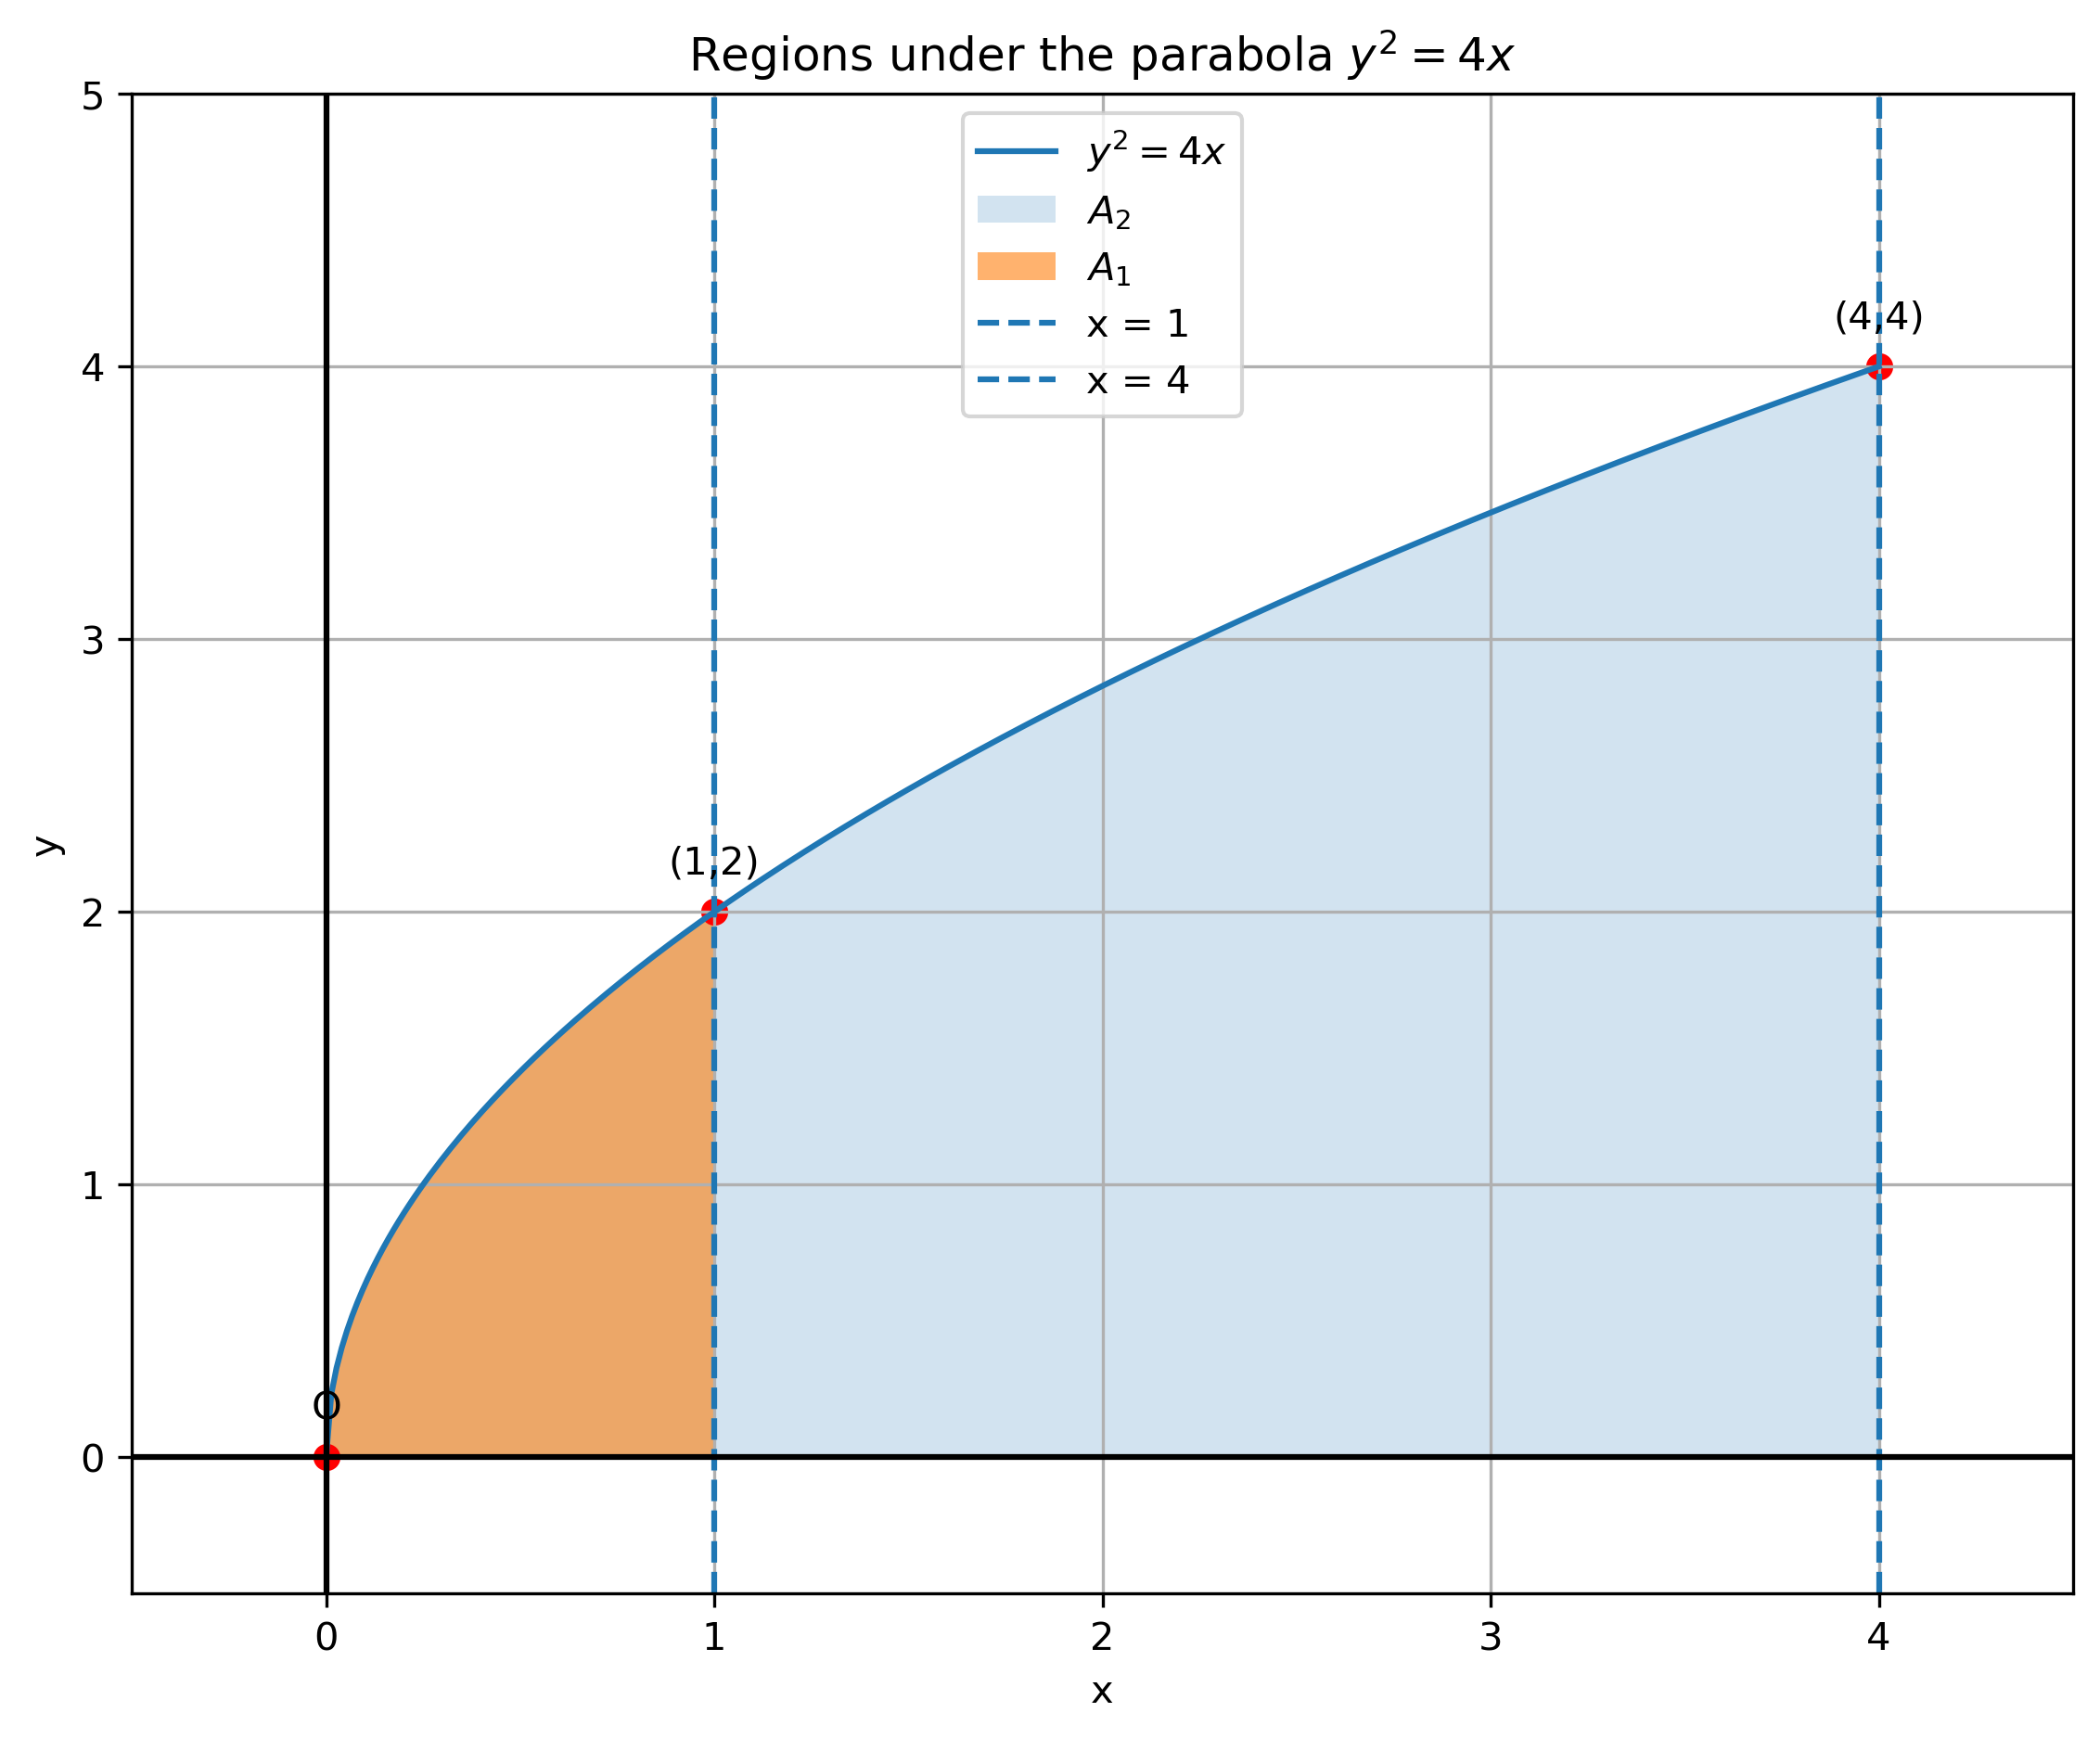
\includegraphics[
                width=0.5\textwidth,
                keepaspectratio
            ]{figs/s1242.png}
        };
    \end{tikzpicture}

\end{figure}

\item
Overspeeding increases fuel consumption and decreases fuel economy as a result of tyre rolling friction and air resistance. While vehicles reach optimal fuel economy at different speeds, fuel mileage usually decreases rapidly at speeds above 80km/h.

\begin{figure}[ht]
    \centering

    \begin{tikzpicture}
        \node[inner sep=0pt] at (0,0)
        {
            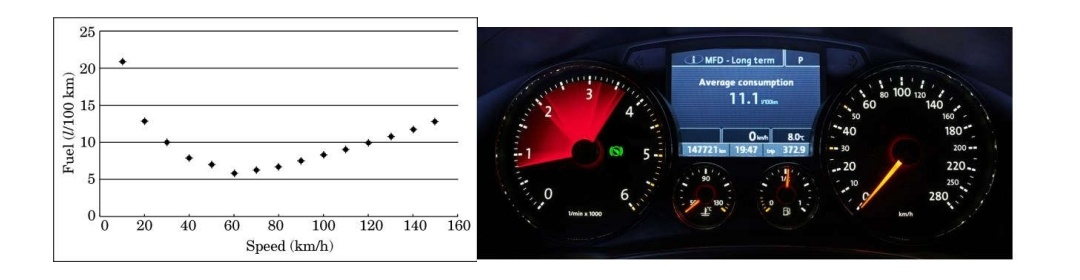
\includegraphics[
                width=\textwidth,
                keepaspectratio
            ]{figs/q1243.png}
        };
    \end{tikzpicture}

\end{figure}
The relation between fuel consumption $F$ $\brak{\text{litres per } 100 \text{km}}$
and speed $V$ \brak{km/h} is given by
\begin{align}
F=\frac{V^2}{500}-\frac{V}{4}+14.
\end{align}

On the basis of the above information,answer the following questions.
\begin{enumerate}

\item Find $F$ when $V=40$ km/h.
\item Find $\dfrac{dF}{dV}$.
\item \brak{a} Find the speed $V$ for which fuel consumption $F$ is minimum.
\item \brak{b} Find the quantity of fuel required to travel $600km$ at the speed V at which $\dfrac{dF}{dV} = -0.01$.

\end{enumerate}

\solution
\brak{i}
Given,
\begin{align}
F=\frac{V^2}{500}-\frac{V}{4}+14.
\end{align}
Substituting $V=40$,
\begin{align}
F=\frac{40^2}{500}-\frac{40}{4}+14.
\end{align}
Simplifying,
\begin{align}
F=\frac{1600}{500}-10+14.
\end{align}
Therefore,
\begin{align}
F=3.2-10+14.
\end{align}
Hence,
\begin{align}
F=7.2\text{ litres per }100\text{ km}.
\end{align}
\brak{ii}
Given,
\begin{align}
F=\frac{V^2}{500}-\frac{V}{4}+14.
\end{align}

Differentiating both sides with respect to $V$,
\begin{align}
\frac{dF}{dV}
=\frac{1}{500}\frac{d}{dV}\brak{V^2}
-\frac{1}{4}\frac{d}{dV}\brak{V}
+\frac{d}{dV}\brak{14}.
\end{align}

Therefore,
\begin{align}
\frac{dF}{dV}
=\frac{2V}{500}-\frac{1}{4}.
\end{align}

Hence,
\begin{align}
\frac{dF}{dV}=\frac{V}{250}-\frac{1}{4}.\label{eq:EE26BTECH11211-Prob_43.10}
\end{align}


\brak{iii}
\\For minimum fuel consumption,
\begin{align}
\frac{dF}{dV}=0.
\end{align}
From \eqref{eq:EE26BTECH11211-Prob_43.10}
\begin{align}
\frac{V}{250}-\frac{1}{4}=0.
\end{align}
Therefore,
\begin{align}
\frac{V}{250}=\frac{1}{4}.
\end{align}
Multiplying both sides by $250$,
\begin{align}
V=\frac{250}{4}.
\end{align}
Hence,
\begin{align}
V=62.5\text{ km/h}.
\end{align}
To verify that the fuel consumption is minimum, differentiate
again:
\begin{align}
\frac{d^2F}{dV^2}=\frac{1}{250}.
\end{align}
Since
\begin{align}
\frac{d^2F}{dV^2}=\frac{1}{250}>0,
\end{align}
the fuel consumption is minimum at $V=62.5$ km/h.
\\Therefore, the required speed is
\begin{align}
V=62.5\text{ km/h}
\end{align}

\brak{iii}
Find the quantity of fuel required to travel $600$ km at the speed
$V$ for which
\begin{align}
\frac{dF}{dV}=-0.01.
\end{align}
From \eqref{eq:EE26BTECH11211-Prob_43.10}
\begin{align}
\frac{dF}{dV}=\frac{V}{250}-\frac{1}{4}.
\end{align}
Given,
\begin{align}
\frac{dF}{dV}=-0.01.
\end{align}
Therefore,
\begin{align}
\frac{V}{250}-\frac{1}{4}=-0.01.
\end{align}
Rearranging,
\begin{align}
\frac{V}{250}=\frac{1}{4}-0.01.
\end{align}
Thus,
\begin{align}
\frac{V}{250}=0.25-0.01=0.24.
\end{align}
Multiplying both sides by $250$,
\begin{align}
V=250\brak{0.24}.
\end{align}
Hence,
\begin{align}
V=60\text{ km/h}.
\end{align}
{Step 2: Calculate fuel consumption at this speed.}

The fuel consumption is
\begin{align}
F=\frac{V^2}{500}-\frac{V}{4}+14.
\end{align}
Substituting $V=60$,
\begin{align}
F=\frac{60^2}{500}-\frac{60}{4}+14.
\end{align}
Simplifying,
\begin{align}
F=\frac{3600}{500}-15+14.
\end{align}
Therefore,
\begin{align}
F=7.2-15+14.
\end{align}
Hence,
\begin{align}
F=6.2\text{ litres per }100\text{ km}.
\end{align}
{Step 3: Calculate the fuel required for $600$ km.}
\\Since
\begin{align}
\text{Fuel required for }100\text{ km}=6.2\text{ litres},
\end{align}
the fuel required for $600$ km is
\begin{align}
\text{Fuel required}=\frac{600}{100}\times 6.2.
\end{align}
Therefore,
\begin{align}
\text{Fuel required}=6\times 6.2.
\end{align}
Hence,
\begin{align}
\text{Fuel required}=37.2\text{ litres}.
\end{align}

{Final Answers:}
\begin{align}
\begin{aligned}
\text{\brak{i}}\quad &F=7.2\text{ litres per }100\text{ km},\\[4pt]
\text{\brak{ii}}\quad &\frac{dF}{dV}=\frac{V}{250}-\frac{1}{4},\\[4pt]
\text{\brak{iii}\brak{a}}\quad &V=62.5\text{ km/h},\\[4pt]
\text{\brak{iii}\brak{b}}\quad &37.2\text{ litres for }600\text{ km}.
\end{aligned}
\end{align}

\item
The month of september is celebrated as the Rashtriya Poshan Maah across the country. Following a healthy and well-balanced diet is crucial in order to supply the body with the proper nutrients it needs. A balanced diet also keeps us mentally fit and promotes improved level of energy.

\begin{figure}[ht]
    \centering

    \begin{tikzpicture}
        \node[inner sep=0pt] at (0,0)
        {
            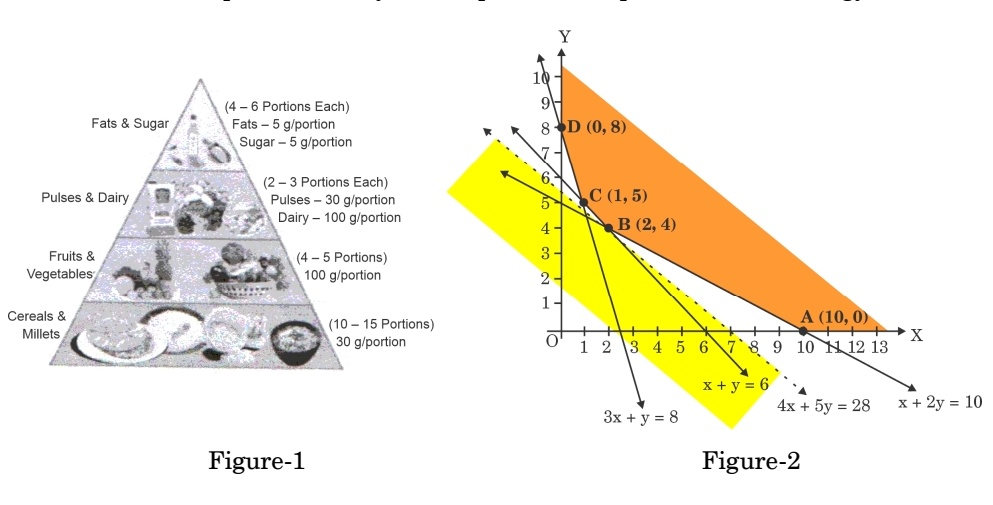
\includegraphics[
                width=\textwidth,
                keepaspectratio
            ]{figs/q1244.png}
        };
    \end{tikzpicture}

\end{figure}
A dietician wishes to minimize the cost of a diet involving two
types of food, food $X$ $\brak{x kg}$ and food $Y$ $\brak{y kg}$, which are
available at the rates of Rs.\ 16/kg and Rs.\ 20/kg, respectively.
The feasible region is shown in Figure 2.

Answer the following questions:

\begin{enumerate}
    \item[\brak{i}] Identify and write all the constraints which determine
    the given feasible region.

    \item[\brak{ii}] If the objective is to minimize the cost
    $Z=16x+20y$, find the values of $x$ and $y$ at which the cost
    is minimum. Also, find the minimum cost, assuming that a minimum
    exists for the given unbounded region.
\end{enumerate}

\solution
{i}
From the given graph, the corner points of the feasible region are
\begin{align}
A\brak{10,0},\quad B\brak{2,4},\quad C\brak{1,5},\quad D\brak{0,8}.
\end{align}
The boundary lines are
\begin{align}
x+2y=10,\\
x+y=6,
\end{align}
and
\begin{align}
3x+y=8.
\end{align}
From the shaded feasible region, the constraints are
\begin{align}
x+2y = 10,\\
x+y = 6,\\
3x+y = 8.
\end{align}
Since the quantities of food cannot be negative,
\begin{align}
x = 0,\qquad y = 0.
\end{align}
Therefore, the required constraints are
\begin{align}
x+2y&= 10,\\
x+y&= 6,\\
3x+y&= 8,\\
x&= 0,\\
y&= 0.
\end{align}

{ii}
The objective function is
\begin{align}
Z=16x+20y.
\end{align}
The corner points of the feasible region are
\begin{align}
A\brak{10,0},\quad B\brak{2,4},\quad C\brak{1,5},\quad D\brak{0,8}.
\end{align}
We calculate the value of $Z$ at each corner point.
\\{At point $A\brak{10,0}$:}
\begin{align}
Z=16\brak{10}+20\brak{0}\\
Z=160
\end{align}
{At point $B\brak{2,4}$:}
\begin{align}
Z=16\brak{2}+20\brak{4}\\
Z=32+80\\
Z=112
\end{align}
{At point $C\brak{1,5}$:}
\begin{align}
Z=16\brak{1}+20\brak{5}\\
Z=16+100.\\
Z=116
\end{align}
{At point $D\brak{0,8}$:}
\begin{align}
Z=16\brak{0}+20\brak{8}\\
Z=160
\end{align}
The results can be summarised in the following table:
\begin{align}
\begin{array}{|c|c|}
\hline
\text{Corner point} & Z=16x+20y\\
\hline
A\brak{10,0} & 160\\
B\brak{2,4} & 112\\
C\brak{1,5} & 116\\
D\brak{0,8} & 160\\
\hline
\end{array}
\end{align}
The smallest value is
\begin{align}
Z_{\min}=112
\end{align}
at the point
\begin{align}
B\brak{2,4}.
\end{align}
{Step 2: Verify the minimum for the unbounded region.}
\\Since the feasible region is unbounded, we verify that a smaller
value of $Z$ is not possible.
\\Suppose
\begin{align}
Z<112.
\end{align}
Then
\begin{align}
16x+20y<112.
\end{align}
Dividing by $4$,
\begin{align}
4x+5y<28.
\end{align}
However, every point in the feasible region satisfies
\begin{align}
4x+5y= 28.
\end{align}
Therefore, no feasible point can satisfy $Z<112$.
\\Hence, $Z=112$ is indeed the minimum cost.
\\The minimum cost is
\begin{align}
Z_{\min}=\text{Rs. }112.
\end{align}
\newpage
\item
Airplanes are by far the safest mode of transportation when the
number of transported passengers are measured against personal injuries and fatality totals.
Previous records state that the  probability of an airplane crash is $0.00001\%$. Further,
there are $95\%$ chances that there will be survivors after a plane crash.
Assume that in case of no crash, all passengers survive.


\begin{figure}[ht]
    \centering

    \begin{tikzpicture}
        \node[inner sep=0pt] at (0,0)
        {
            
\includegraphics[
                width=0.5\textwidth,
                keepaspectratio
            ]{figs/q1245.png}
        };
    \end{tikzpicture}

\end{figure}
Let $E_1$ be the event that there is a plane crash, $E_2$ be the
event that there is no crash. Let $A$ be the event that passengers
survive after the journey.

\solution
\brak{i} Find the probability that the airplane will not crash.

Given,
\begin{align}
P\brak{E_1}=0.00001\%.
\end{align}
Converting the percentage into a probability,
\begin{align}
P\brak{E_1}=\frac{0.00001}{100}=10^{-7}.
\end{align}
Since $E_2$ is the complement of $E_1$,
\begin{align}
P\brak{E_2}=1-P\brak{E_1}.
\end{align}
Therefore,
\begin{align}
P\brak{E_2}=1-10^{-7}.
\end{align}
Hence,
\begin{align}
P\brak{E_2}=0.9999999
\end{align}

\brak{ii} Find $P\brak{A\mid E_1}+P\brak{A\mid E_2}$.

\solution
The probability of passengers surviving given that a crash occurs
is
\begin{align}
P\brak{A\mid E_1}=95\%=0.95.
\end{align}
If there is no crash, all passengers survive. Therefore,
\begin{align}
P\brak{A\mid E_2}=1.
\end{align}
Hence,
\begin{align}
P\brak{A\mid E_1}+P\brak{A\mid E_2}=0.95+1.
\end{align}
Thus,
\begin{align}
P\brak{A\mid E_1}+P\brak{A\mid E_2}=1.95
\end{align}

\brak{iii}\brak{a} Find $P\brak{A}$.

\solution
Using the law of total probability,
\begin{align}
P\brak{A}=P\brak{E_1}P\brak{A\mid E_1}+P\brak{E_2}P\brak{A\mid E_2}.
\end{align}
Substituting the known values,
\begin{align}
P\brak{A}=10^{-7}\brak{0.95}+\brak{1-10^{-7}}\brak{1}.
\end{align}
Expanding,
\begin{align}
P\brak{A}=0.95\times10^{-7}+1-10^{-7}.
\end{align}
Therefore,
\begin{align}
P\brak{A}=1-0.05\times10^{-7}.
\end{align}
Hence,
\begin{align}
P\brak{A}=1-5\times10^{-9}.
\end{align}

\brak{iii}\brak{b} Find $P\brak{E_2\mid A}$ 

\solution
Using Bayes' theorem \label{eq:EE26BTECH11211-Prob_16},
\begin{align}
P\brak{E_2\mid A}
=\frac{P\brak{E_2}P\brak{A\mid E_2}}{P\brak{A}}.
\end{align}
From the previous parts,
\begin{align}
P\brak{E_2}=1-10^{-7},
\qquad P\brak{A\mid E_2}=1,
\end{align}
and
\begin{align}
P\brak{A}=1-5\times10^{-9}.
\end{align}
Substituting,
\begin{align}
P\brak{E_2\mid A}
=\frac{1-10^{-7}}{1-5\times10^{-9}}.
\end{align}
Therefore,
\begin{align}
P\brak{E_2\mid A}
=\frac{1-10^{-7}}{1-5\times10^{-9}}
\end{align}

\end{enumerate}

